\documentclass[12pt, openany, oneside, a4paper, english, brazil]{abntex2}   % Padrão Abntex2

%***************************** PACOTES *********************************** %
\usepackage{color,graphicx}

%\usepackage[within=none]{newfloat}
\usepackage[utf8]{inputenc}		     % Codificacao do documento (conversão automática dos acentos)


%	Fonte
\usepackage[T1]{fontenc}		   	 % Selecao de codigos de fonte.
\usepackage[brazil]{babel}
\usepackage{lmodern}			     % Usa a fonte Latin Modern

%	Matemático e Gráfico
\usepackage{float}
\usepackage{graphics,graphicx}	     % pacotes para inserir figuras .eps ou .jpg
\graphicspath{{figuras/}}            % pasta de figuras
\usepackage{amssymb}           		 % pacote para fontes e simbolos matemáticos
\usepackage{longtable}          	 % possibilita inserir grandes tabelas
\usepackage{makecell}                % possibilita pular linhas nas tabelas
\usepackage{xcolor,colortbl,multirow} % permite textos e tabelas com cores
\usepackage{amsmath}           		 % pacote para equações
\usepackage{epstopdf}
\usepackage{ragged2e}
\usepackage{listings}
%\lstset{numbers=left, numberstyle=\tiny, stepnumber=1, numbersep=5pt, basicstyle=\scriptsize ,frame=tbrl}
\usepackage{etoolbox}
\usepackage{multicol}
%\usepackage{caption}
\usepackage[position=b,singlelinecheck=on]{subfig}

\floatstyle{plaintop}
\newfloat{quadro}{htbp}{loq}
\floatname{quadro}{Quadro}

\makeatletter
\patchcmd{\listof}% <cmd>
{\float@listhead}% <search>
{\@namedef{l@#1}{\l@table}\float@listhead}% <replace>
{}{}% <success><failure>
\makeatother

%\makeatletter
%\renewcommand*{\float@listhead}[1]{%
%	\@ifundefined{chapter}{%
%		\section*{#1}%
%		\addcontentsline{toc}{section}{#1}%
%	}{%
%	\chapter*{#1}% 
%	\addcontentsline{toc}{chapter}{#1}%
%}%
%\@mkboth{\MakeUppercase{#1}}{\MakeUppercase{#1}}%
%}
%\makeatother




%\DeclareFloatingEnvironment{quadro}[Quadro][Lista de quadros]
%\DeclareCaptionType{quadro}[Quadros][Lista de quadros]


% % % % % % % % % % % % % % % % % % % %

\definecolor{codegreen}{rgb}{0,0.6,0}
\definecolor{codegray}{rgb}{0.5,0.5,0.5}
\definecolor{codepurple}{rgb}{0.58,0,0.82}
\definecolor{backcolour}{rgb}{0.95,0.95,0.92}

%\definecolor{verde}{rgb}{0,0,0}

\lstdefinestyle{mystyle}{
	backgroundcolor=\color{backcolour},   
	commentstyle=\color{codegreen},
	keywordstyle=\color{magenta},
	numberstyle=\tiny\color{codegray},
	stringstyle=\color{codepurple},
	basicstyle=\footnotesize,
	breakatwhitespace=false,         
	breaklines=true,                 
	captionpos=b,                    
	keepspaces=true,                 
	numbers=left,                    
	numbersep=5pt,                  
	showspaces=false,                
	showstringspaces=false,
	showtabs=false,                  
	tabsize=2
}

\lstset{style=mystyle}

%	Estrutural
\usepackage{url}
\usepackage{threeparttable}     	 % permite a inserção de notas de rodapé nas tabelas
\usepackage{lscape}             	 % orientação de página LANDSCAPE
\usepackage{pifont}             	 % acrescenta símbolos diferentes.
%\usepackage{cmap}					 % Mapear caracteres especiais no PDF	
\usepackage{lastpage}				 % Usado pela Ficha catalográfica
\usepackage{indentfirst}			 % Indenta o primeiro parágrafo de cada sessão.



% Pacotes de citações
\usepackage[brazilian,hyperpageref]{backref}	 % Paginas com as citações na bibl
\usepackage[alf]{abntex2cite}	% Citações padrão ABNT numerica
     
% remover bordas dos links
\hypersetup{
    colorlinks,
    linkcolor={black},
    citecolor={black},
    urlcolor={black}
} % resto dos pacotes Latex
%\usepackage[english]{style/UCSAL-Template} % personalização da ABNTEX2 para escrita em inglês
\usepackage[portuguese]{style/ucsal} % personalização da ABNTEX2 para escrita em português
\usepackage{longtable}
\usepackage{blindtext}
\DisemulatePackage{setspace}
\usepackage{setspace}
\usepackage{lipsum}
\usepackage[left=3cm,top=3cm,right=2cm,bottom=2cm]{geometry}
\usepackage{fontspec}
\setmainfont{Arial}

% --- Entrega 2: diagramas, listagens e marcador de pendências ---
\usepackage{tikz}
\usetikzlibrary{arrows.meta,positioning,shapes.geometric}
\newcommand{\diagrama}[3]{\IfFileExists{figuras/#1.png}{\includegraphics[#2]{figuras/#1.png}}{\IfFileExists{figuras/#1.pdf}{\includegraphics[#2]{figuras/#1.pdf}}{\fbox{\parbox{0.92\textwidth}{\centering\vspace{1.2cm}\textcolor{red!70!black}{\textbf{[DIAGRAMA PENDENTE: \detokenize{figuras/#1.png}]}}\\[3pt]\small #3\vspace{1.2cm}}}}}} % espaço reservado até existir o arquivo
\newcommand{\pendente}[1]{\textcolor{red!70!black}{\textbf{[PENDENTE: #1]}}} % remover antes da entrega final


%inserindo apenas uma página

%---------------------------------------------------------------
%--------- DADOS BÁSICOS DO TRABALHO (Preencher todos) ---------
%---------------------------------------------------------------


\titulo{Segurança e Governança de Dados com uso de LLMs no Desenvolvimento de Software}   % Título do Trabalho em Português

\tituloingles{Study of the need to insert programming education in secondary and elementary education} % Título do Trabalho em Inglês

\palavraschave{SEU TEMA}  % 5 palavras-chave

\keywords{1. Programming teaching. 2. Young people's lack of IT information. 3. Need of the IT job market.}   % 5 palavras-chave para resumo em inglês

%\DEELautor{{ALUNO} {\\ aluno2 }}   %Aluno autor do trabalho
%
%}

\autor{Bruno Dantas de Oliveira \\ Zaira Dutra Pinto Souza \\ Gustavo Ricci Ferreira \\ Matheus Pires Fraga \\ Caio Caldas Matos de Morais}
\curso{Bacharelado em Engenharia de Software}												
\orientador{Prof. Sheila Tirony}  % Professor Orientador membro da banca 

\membrob{Prof. Me. Segundo professor}   % Professor membro da banca 
\membroc{Prof. Me. Terceiro professor}   % Professor membro da banca

\local{Salvador}   % Cidade da instituição
\data{2022}        % Ano de realização

%--------------------------------------------------------------------------------------------



\begin{document}
\onehalfspacing

% Seleção automática do idioma, não alterar
\ifx\isenglish\undefined
    \selectlanguage{brazil}
\else
    \selectlanguage{english}
\fi

% Texto da Dedicatória (OBS: dedicatória é opcional)
% Caso não queira inserir, deixe em branco ( \dedicatoria{} )
\DEELdedicatoria{Dedico este trabalho a todos aqueles.... \\}  
    
% Texto dos Agradecimentos (OBS: Agradecimentos é opcional)
% Caso não queira inserir, deixe em branco ( \agradecimentos{} )
\DEELagradecimentos{Agradeço primeiramente a ... } 

                       
% Texto da Epígrafe (OBS: Epígrafe é opcional)
% Caso não queira inserir, deixe em branco ( \epigrafe{} )
\DEELepigrafe{\textit{"ABC"} \\ (Albert Einstein)} 
    

% Texto do Resumo (OBS: Resumo é Obrigatório)
\DEELresumo{XXXXX .
 } 
     
% Texto do Abstract (OBS: Abstract é Obrigatório)
\DEELabstract{ESCREVA AQUI SEU RESUMO em INGLES
} 
    



%%%%%%%%%%%%%%%%%%%%%%%%%%%
%% Elementos Pré-Textuais%%
%%%%%%%%%%%%%%%%%%%%%%%%%%%
\ElementosPreTextuais
% Insere todos os elementos Pré-Textuais listados (capa, folha de rosto, ...)
    % capa                   % Obrigatório
    % folhaderosto           % Obrigatório
    % folhaaprovacao         % Obrigatório
	% dedicatoria            % Opcional
	% agradecimentos         % Opcional
    % epigrafe               % Opcional
    % resumo                 % Obrigatório
    % abstract               % Obrigatório

%\newpage
%--------Lista de figuras--------
\ListaDeFiguras 
%--------Lista de tabelas--------
\ListaDeTabelas 
%--------Lista de Siglas e Abreviaturas--------
%----------Lista de Acronimos --------------------------------
\ifx\isenglish\undefined
\pretextualchapter{Lista de Siglas e Abreviaturas}
\else
\pretextualchapter{Acronyms}
\fi


%\renewcommand{\baselinestretch}{2} %espaçamento entre linhas (por definicçào, no espABNT é 2)
\begin{tabbing}
xxxxxxxxxxx \= xxxxxxxxxxxxx \kill
\textsc{API}            \> \textit{Application Programming Interface}\\


\textsc{BES}            \> Bacharelado em Engenharia de Software\\
\textsc{CA}            \> \textit{Certificate Authority} (autoridade certificadora)\\
\textsc{CI}            \> \textit{Continuous Integration} (integração contínua)\\
\textsc{CLI}            \> \textit{Command-Line Interface} (interface de linha de comando)\\
\textsc{HTTP}            \> \textit{Hypertext Transfer Protocol}\\
\textsc{HTTPS}            \> \textit{HTTP Secure}\\
\textsc{JSON}            \> \textit{JavaScript Object Notation}\\
\textsc{LLM}            \> \textit{Large Language Model} (modelo de linguagem de grande escala)\\
\textsc{MITM}            \> \textit{Man-in-the-Middle}\\
\textsc{MoSCoW}            \> \textit{Must, Should, Could, Won't} (técnica de priorização)\\
\textsc{PEM}            \> \textit{Privacy-Enhanced Mail} (formato de certificados e chaves)\\
\textsc{RF}            \> Requisito funcional\\
\textsc{RNF}            \> Requisito não funcional\\
\textsc{SGBD}            \> Sistema gerenciador de banco de dados\\
\textsc{TLS}            \> \textit{Transport Layer Security}\\
\textsc{TUI}            \> \textit{Terminal User Interface} (interface de terminal)\\
\textsc{UC}            \> Caso de uso\\
\textsc{YAML}            \> \textit{YAML Ain't Markup Language}

\end{tabbing}

%\addcontentsline{toc}{chapter}{Lista de Siglas e Abreviaturas}
   
%--------Lista de Simbolos e Notação--------
%\include{list_simbolos} 
%--------Sumário-------
\Sumario


%%%%%%%%%%%%%%%%%%%%%%
%%Elementos Textuais%%
%%%%%%%%%%%%%%%%%%%%%%
\textual 
\chapter{Introdução}\label{chp:intro}

Assistentes de programação baseados em modelos de linguagem de grande escala (\textit{Large Language Models}, LLMs) tornaram-se parte do cotidiano do desenvolvimento de software. Integrados a editores, a ambientes de desenvolvimento e à linha de comando, eles completam código, sugerem refatorações e respondem a perguntas sobre o projeto. Para isso precisam de contexto: a cada interação, trechos de código, arquivos abertos, mensagens de erro e, com frequência, arquivos de configuração são enviados a provedores externos de inteligência artificial, fora do domínio de controle da organização que utiliza a ferramenta.

Esse fluxo cria uma superfície de exposição de dados que os controles de segurança tradicionais tratam mal. O dado sensível não é subtraído por um atacante: é enviado, de forma legítima e muitas vezes inadvertida, pela própria ferramenta autorizada a um destino também autorizado (Capítulo~\ref{chp:fund}). Credenciais de acesso, chaves de API, \textit{tokens} e identificadores internos que acompanham o contexto passam, assim, a residir na infraestrutura de terceiros. Casos reais indicam a dimensão do problema: em 2023, engenheiros da \textit{Samsung} submeteram código-fonte proprietário a um assistente de IA generativa, o que resultou em três incidentes de vazamento em cerca de um mês e na proibição da ferramenta pela empresa; e relatórios recentes de monitoramento de segredos apontam volume crescente de credenciais expostas em repositórios públicos, inclusive em arquivos de configuração ligados a ferramentas de IA.

Diante desse quadro, as organizações tendem a oscilar entre proibir o uso das ferramentas, abrindo mão de seus ganhos de produtividade, e aceitar o risco. Entre os dois extremos há espaço para mecanismos técnicos que permitam usar o assistente sem que o segredo chegue ao provedor. A literatura revisada neste trabalho oferece peças desse mecanismo, mas não o conjunto: há métodos de detecção de segredos e de dados pessoais avaliados sobre artefatos estáticos, técnicas de preservação de privacidade aplicadas ao treinamento ou à arquitetura interna do agente, e assistentes executados localmente que dispensam o provedor externo. Não foi identificado, entre os trabalhos analisados, um que combine a interceptação do tráfego em tempo real, a independência em relação à ferramenta e ao provedor, e a avaliação do impacto operacional da camada de proteção (Capítulo~\ref{chp:fund}). É nessa lacuna que este trabalho se situa.

\section{Problema de Pesquisa}
\label{sec:intro_problema}

O problema que orienta este trabalho pode ser formulado da seguinte maneira: \textit{como impedir que dados sensíveis presentes no contexto enviado por ferramentas de desenvolvimento assistidas por LLM cheguem a provedores externos de IA, sem exigir a substituição da ferramenta nem do provedor e sem degradar de forma perceptível a experiência do desenvolvedor?}

Esse problema se desdobra nas questões de pesquisa (\textit{Research Questions}, RQs) da Tabela~\ref{tab:rqs}, cada uma associada a uma das cadeias de busca da revisão sistemática descrita no Capítulo~\ref{chp:met}. As quatro primeiras são respondidas pela revisão da literatura (Capítulo~\ref{chp:fund}); a quinta é respondida, também, pela verificação experimental do mecanismo proposto (Capítulos~\ref{chp:test} e~\ref{chp:res}).

\begin{table}[htb]
\centering
\caption{Questões de pesquisa}\label{tab:rqs}
\small
\begin{tabular}{|p{1.1cm}|p{9.3cm}|p{1.6cm}|p{2.6cm}|}
\hline
\textbf{ID} & \textbf{Questão} & \textbf{Cadeia} & \textbf{Respondida em} \\ \hline
RQ1 & Que riscos de exposição de dados, código e privacidade o uso de assistentes de programação baseados em LLM introduz? & A & Cap.~\ref{chp:fund} \\ \hline
RQ2 & Que técnicas de sanitização, redação e anonimização são empregadas para remover ou substituir informação sensível antes do envio ao modelo? & B & Cap.~\ref{chp:fund} \\ \hline
RQ3 & Que arquiteturas intermediárias (\textit{proxies}, \textit{gateways}, \textit{middlewares}) são utilizadas para prevenir a perda de dados? & C & Cap.~\ref{chp:fund} \\ \hline
RQ4 & Que métodos permitem detectar credenciais, segredos e dados pessoais em código e em ambientes de desenvolvimento? & D & Cap.~\ref{chp:fund} \\ \hline
RQ5 & Qual é o impacto operacional (latência, utilidade, produtividade) de introduzir uma camada de proteção nesse fluxo? & E & Cap.~\ref{chp:fund}, \ref{chp:test} e~\ref{chp:res} \\ \hline
\end{tabular}
\fonte{Elaborado pela equipe (2026), a partir das cadeias de busca da Seção~\ref{sec:strings_busca}.}
\end{table}

\section{Justificativa}

\textbf{Do ponto de vista prático}, o uso de assistentes de código já é decisão consolidada em muitas equipes, de modo que a alternativa de eliminar o provedor externo (como em assistentes locais) nem sempre está disponível. Uma camada de proteção que atue sobre o tráfego, sem alterar a ferramenta do desenvolvedor, reduz o custo de adoção e permite que a política de dados da organização seja aplicada, e não apenas declarada.

\textbf{Do ponto de vista científico}, a revisão da literatura mostra que as abordagens existentes avaliam a detecção sobre artefatos estáticos ou atuam no treinamento do modelo, e que a latência introduzida por uma camada de proteção não é avaliada nos estudos analisados. O trabalho contribui ao propor um mecanismo que opera sobre o tráfego em trânsito e ao reportar medições do seu custo operacional.

\textbf{Do ponto de vista social e de governança}, o mecanismo gera uma trilha de auditoria que registra o que foi detectado sem armazenar o conteúdo das requisições, o que oferece à organização evidência para acompanhar o uso das ferramentas de IA. Por ser distribuído como \textit{software} de código aberto, o resultado pode ser examinado, reproduzido e evoluído por terceiros.

\section{Objetivos}
\label{sec:intro_obj}

\subsection{Objetivo Geral}

Projetar, implementar e avaliar um mecanismo de \textit{proxy} intermediário, independente da ferramenta e do provedor, capaz de detectar e redigir dados sensíveis no tráfego HTTP enviado por ferramentas de desenvolvimento assistidas por LLM a provedores externos de IA, e avaliar o seu impacto operacional.

\subsection{Objetivos Específicos}

\begin{enumerate}
    \item[\textbf{OE1.}] Identificar, por meio de revisão sistemática da literatura, os riscos de exposição de dados no uso de assistentes de programação baseados em LLM e as técnicas existentes de detecção, sanitização e proteção por arquiteturas intermediárias, caracterizando as lacunas a que o trabalho responde.
    \item[\textbf{OE2.}] Levantar e especificar os requisitos funcionais e não funcionais do mecanismo, identificando seus usuários e definindo critérios de aceitação mensuráveis sempre que possível.
    \item[\textbf{OE3.}] Projetar a arquitetura, o modelo de dados e as interfaces do mecanismo, documentando-os em diagramas.
    \item[\textbf{OE4.}] Implementar o mecanismo de forma incremental e em código aberto, registrando as decisões técnicas e mantendo a documentação atualizada.
    \item[\textbf{OE5.}] Verificar a eficácia da detecção e da redação, considerando a detecção dos formatos de credencial suportados, a ausência de falsos positivos nos casos de teste e a integridade das requisições encaminhadas.
    \item[\textbf{OE6.}] Avaliar o impacto operacional do mecanismo, medindo a latência e a vazão da análise para corpos de requisição de diferentes tamanhos.
\end{enumerate}

\section{Delimitação do Escopo}

O trabalho trata dos dados que saem da máquina do desenvolvedor em requisições HTTP(S) dirigidas a provedores de IA. A detecção baseia-se em padrões (expressões regulares e valores literais) voltados principalmente a credenciais de formato conhecido, configuráveis pelo usuário. Ficam fora do escopo: o treinamento ou o ajuste fino de modelos; a inspeção das respostas dos provedores; a classificação semântica de conteúdo e a detecção de código proprietário por similaridade; a avaliação da qualidade das respostas do LLM após a redação; e a demonstração de conformidade com normas específicas de proteção de dados. As consequências dessas delimitações são discutidas no Capítulo~\ref{chp:res}.

\section{Procedimentos Metodológicos}

Trata-se de pesquisa aplicada, de natureza tecnológica, composta por três frentes. A primeira é uma revisão sistemática da literatura, conduzida com cinco cadeias de busca na base IEEE Xplore e triada com apoio da ferramenta Parsifal, que resultou em oito trabalhos incluídos entre quinze trabalhos únicos analisados (Capítulos~\ref{chp:met} e~\ref{chp:fund}). A segunda é o desenvolvimento incremental do mecanismo, precedido do levantamento de requisitos e do projeto da solução e acompanhado do registro das decisões técnicas (Capítulos~\ref{chp:req} a~\ref{chp:dev}). A terceira é a verificação do mecanismo por testes automatizados, de integração e de desempenho (Capítulo~\ref{chp:test}), cujos resultados são analisados à luz dos objetivos no Capítulo~\ref{chp:res}.

\section{Estrutura do Trabalho}

Além desta introdução, o trabalho está organizado em oito capítulos. O Capítulo~\ref{chp:fund} apresenta a fundamentação teórica e os trabalhos relacionados. O Capítulo~\ref{chp:met} descreve a metodologia da revisão. Os Capítulos~\ref{chp:req}, \ref{chp:proj} e~\ref{chp:dev} documentam o levantamento de requisitos, o projeto e o desenvolvimento da solução. O Capítulo~\ref{chp:test} reúne o planejamento, a execução e os resultados dos testes. O Capítulo~\ref{chp:res} apresenta o produto, os resultados e sua discussão, a comparação com os objetivos e as limitações. O Capítulo~\ref{chp:conc} apresenta as conclusões, as contribuições e as recomendações para trabalhos futuros.
 % Texto do cap1.tex
\chapter{Fundamentação Teórica}\label{chp:fund}

Esta seção apresenta uma breve fundamentação téorica sobre.......

\section{Segurança e Vazamento de Dados no Desenvolvimento Assistido por IA}

A adoção de ferramentas de desenvolvimento assistidas por modelos de linguagem de grande escala introduz uma nova superfície de exposição de dados: cada interação entre o desenvolvedor e o assistente, seja um trecho de código, uma mensagem de commit ou o contexto de um arquivo aberto no editor é enviada a um provedor externo de inteligência artificial para ser processada. Esse fluxo caracteriza o que a literatura denomina \textit{data leakage}, definido como a transmissão não autorizada ou não intencional de informação sensível para fora do domínio de controle da organização, e sua variação mais específica ao contexto deste trabalho, o \textit{code leakage}, que se refere à exposição de código-fonte proprietário, segredos de aplicação e credenciais de acesso durante o uso de ferramentas externas de desenvolvimento.

Diferentemente de vazamentos causados por falhas de configuração de infraestrutura ou ataques direcionados, a exposição de dados em ferramentas assistidas por LLM ocorre como efeito colateral do uso legítimo da ferramenta: o dado sensível não é roubado, é enviado voluntariamente pelo próprio usuário como parte do fluxo normal de trabalho, o que torna esse risco mais difícil de mitigar por controles de segurança perimetrais tradicionais, uma vez que o tráfego se origina de dentro do ambiente de desenvolvimento e é direcionado a um destino legítimo e autorizado pela organização.

Como o ocorrido na empresa \textit{Samsung} em 2023, onde os seus engenheiros usaram o \textit{ChatGPT} para avaliar o código-fonte e otimizar as sequências de testes para identificar falhas nos chips que estavam projetando. Causando três situações de vazamento de dados no intervalo de um mês, culminando na proibição do uso da ferramenta pelos funcionários da empresa e na discussão de formas seguras de utilização.

Em 2026, a ferramenta de detecção de segredos \textit{GitGuardian}, da plataforma \textit{GitHub}. Registrou aproximadamente 29 milhões de chaves, tokens e credenciais expostas. E mais de 24.000 segredos únicos em arquivos de configuração MCP no GitHub público. Reforçando o fato de que o uso irrestrito das ferramentas trazem riscos a segurança. 


\section{Modelos de Linguagem de Grande Escala (LLMs) e Riscos de Privacidade}

Modelos de linguagem de grande escala (LLMs) são sistemas de aprendizado profundo treinados sobre grandes volumes de texto, capazes de gerar e interpretar linguagem natural e código-fonte a partir de um contexto (\textit{prompt}) fornecido pelo usuário. No cenário de ferramentas de desenvolvimento assistidas por IA, esse contexto tipicamente inclui não apenas a instrução explícita do usuário, mas também trechos do código-fonte do projeto, estrutura de arquivos e, em alguns casos, o histórico de interações anteriores, dados que trafegam até a infraestrutura do provedor do modelo, frequentemente hospedada por terceiros e fora do domínio de controle direto da organização que utiliza a ferramenta.

\citeonline{xu2025privacypreserving} sistematizam os principais vetores de risco à privacidade decorrentes desse fluxo, categorizando-os em riscos durante o treinamento do modelo, quando dados sensíveis podem ser memorizados e posteriormente reproduzidos, e riscos durante a inferência, quando o próprio conteúdo do prompt enviado pelo usuário constitui a superfície de exposição. Os autores destacam que técnicas de computação segura, como criptografia homomórfica, ambientes de execução confiável (TEE) e computação multipartidária segura (MPC), têm sido propostas para mitigar esses riscos, ainda que com custos computacionais e de latência relevantes para cenários de uso interativo. Em linha semelhante, \citeonline{zhang2024privacyasst} argumentam que, em arquiteturas de agentes que utilizam ferramentas externas, o risco de exposição se amplia porque o agente frequentemente repassa dados do usuário não apenas ao modelo de linguagem, mas também às ferramentas que ele orquestra como motores de busca, interpretadores de código e integrações com sistemas de terceiros, multiplicando os pontos de possível vazamento.

\section{Assistentes de Desenvolvimento (Code Assistants)}

Assistentes de desenvolvimento baseados em IA (\textit{code assistants}) são ferramentas integradas ao ambiente de desenvolvimento (IDE) ou à linha de comando que utilizam LLMs para auxiliar tarefas como completude de código, geração de funções, refatoração e revisão. Para operar de forma útil, esses assistentes precisam de acesso ao contexto do projeto, arquivos abertos, estrutura de diretórios, histórico de versionamento, e esse contexto é, em arquiteturas convencionais baseadas em provedores de nuvem, transmitido integralmente ao provedor externo a cada interação.

\citeonline{elatrassi2025codewisp} ilustram uma abordagem arquitetural alternativa a esse modelo com o \textit{CodeWisp}, um assistente de código que opera localmente, utilizando geração aumentada por recuperação (RAG) com indexação semântica guiada por árvore de sintaxe abstrata (AST) para localizar e fornecer apenas os trechos de código relevantes ao contexto da tarefa, sem depender de um LLM hospedado externamente. Embora a proposta demonstre viabilidade técnica, com recall de 0,96 e \textit{Mean Reciprocal Rank} de 0,95 em tarefas de completude, ela pressupõe a substituição do provedor externo por um modelo local, o que não se aplica a cenários em que o uso de LLMs de terceiros (como os grandes provedores comerciais) já está consolidado como decisão de produto ou de negócio da organização.

\section{Detecção de Dados Sensíveis}

A detecção de dados sensíveis é o processo de identificar, em um fluxo de texto ou código, elementos que representam informação confidencial, credenciais de acesso, chaves de API, dados pessoalmente identificáveis (PII) ou segredos de aplicação, antes que esse conteúdo seja transmitido a um destino não confiável. As abordagens de detecção evoluíram de técnicas baseadas puramente em expressões regulares e análise de entropia, que apresentam alta taxa de falsos positivos por não considerarem o contexto semântico do conteúdo analisado, para abordagens híbridas e baseadas em aprendizado de máquina.

\citeonline{rahman2025secret} demonstram essa evolução ao combinar extração de candidatos via regex com classificação por modelos de linguagem ajustados (LLaMA-3.1 8B e Mistral-7B), alcançando F1-score de 0,9852 na tarefa de classificação binária de segredos em código-fonte. \citeonline{tsebak2025enhancing} seguem abordagem semelhante ao integrar um modelo transformer contextual (CodeBERT) a um classificador de gradient boosting (XGBoost), reportando redução significativa de falsos positivos frente a métodos tradicionais de entropia. No contexto de dados pessoais em vez de segredos técnicos, \citeonline{sakapertana2025advancing} comparam algoritmos clássicos de aprendizado supervisionado, SVM e Naive Bayes para detecção de PII em respostas de API REST, com SVM atingindo 80,96\% de acurácia, enquanto \citeonline{khan2025aipowered} propõem o uso de modelos generativos em regime \textit{zero-shot}, capazes de se adaptar a novos critérios de sensibilidade sem necessidade de reentreinamento, uma característica relevante para cenários em que a definição do que constitui "dado sensível" pode variar entre organizações.

\section{Mitigação: Sanitização e Redação de Dados}

Uma vez detectado, o dado sensível precisa ser tratado antes de prosseguir ao destino externo. A literatura de privacidade descreve um espectro de técnicas de mitigação: a \textit{redação} (\textit{redaction}), que consiste na remoção ou ocultação total do dado sensível identificado; a \textit{sanitização} (\textit{sanitization}), termo mais amplo que engloba qualquer transformação do conteúdo para reduzir seu risco antes da transmissão; e a \textit{anonimização} e \textit{pseudonimização}, que substituem o valor original por um identificador não reversível ou reversível apenas sob controle específico, respectivamente, permitindo preservar a utilidade estrutural do dado sem expor seu valor real.

\citeonline{zhang2024privacyasst} aplicam esse princípio no nível arquitetural, propondo um mecanismo de embaralhamento (\textit{shuffling}) de atributos combinado a criptografia homomórfica para que agentes de LLM operem sobre dados protegidos sem acesso ao valor original do usuário. \citeonline{pan2025selective} tratam a mitigação em outro ponto do ciclo de vida do modelo, aplicando ruído customizado a tokens privados durante o processo de ajuste fino (\textit{fine-tuning}) em cenários de aprendizado federado, de forma seletiva, isto é, calibrando o nível de proteção conforme a sensibilidade de cada token, em vez de aplicar uma transformação uniforme a todo o conteúdo. Essa noção de seletividade é particularmente relevante para o mecanismo proposto neste trabalho, pois a redação indiscriminada de todo o tráfego comprometeria a utilidade do assistente de código para o desenvolvedor.

\section{Arquiteturas Intermediárias de Proteção}

Arquiteturas de proteção posicionadas entre o cliente e o serviço externo, como \textit{proxies} reversos, \textit{API gateways} e \textit{middlewares}, constituem um padrão consolidado em segurança de aplicações para implementar pontos de aplicação de política (\textit{policy enforcement points}), nos quais regras de segurança, autenticação e inspeção de conteúdo podem ser aplicadas de forma centralizada e transparente às aplicações que consomem o serviço, sem exigir alterações no código-cliente.

\section{Avaliação de Impacto Operacional}

A introdução de qualquer mecanismo de inspeção ou transformação de tráfego entre o cliente e o provedor externo tem potencial de impactar a experiência de uso da ferramenta, seja por meio do aumento de latência introduzido pelo processamento adicional, seja pela redução de utilidade quando o mecanismo de proteção remove ou distorce informação relevante ao funcionamento correto do assistente. A avaliação desse impacto operacional, portanto, não pode se limitar a métricas de eficácia da detecção como precisão e revocação, devendo incorporar também métricas de eficiência, como tempo de resposta e taxa de falsos positivos, que representam o custo prático de se utilizar o mecanismo de proteção no dia a dia do desenvolvedor.

Os trabalhos revisados na Seção 3.4 fornecem parâmetros de referência para essa avaliação: \citeonline{rahman2025secret} e \citeonline{tsebak2025enhancing} reportam F1-score e taxa de falsos positivos como métricas centrais de eficácia de seus classificadores, enquanto a redução de falsos positivos é tratada por \citeonline{tsebak2025enhancing} como requisito prático para viabilizar a adoção da ferramenta em fluxos de trabalho reais, um paralelo direto ao critério de usabilidade que este trabalho pretende avaliar para o mecanismo de proxy proposto. Nenhum dos trabalhos revisados, no entanto, avalia explicitamente a métrica de latência introduzida pelo mecanismo de proteção, o que reforça a avaliação de impacto operacional como uma contribuição relevante deste trabalho frente à literatura atual.

\section{Governança de Dados e IA}

Governança de dados refere-se ao conjunto de políticas, papéis, processos e controles que definem como os dados de uma organização são geridos, protegidos e utilizados ao longo de seu ciclo de vida. No contexto de adoção de ferramentas de IA generativa no desenvolvimento de software, a governança se materializa na definição de quais categorias de dados podem ou não ser enviadas a provedores externos, em quais condições, e sob qual mecanismo de controle e auditoria essa política é efetivamente aplicada, e não apenas declarada.

\citeonline{xu2025privacypreserving} situam esse desafio ao observar que técnicas de computação segura, embora tecnicamente eficazes, ainda carecem de mecanismos maduros de integração com políticas de governança organizacionais em escala, o que limita sua adoção prática fora de ambientes controlados de pesquisa. \citeonline{pan2025selective} ilustram, por outro lado, como decisões de governança podem ser incorporadas diretamente ao mecanismo técnico de proteção, ao permitir que o nível de proteção aplicado a cada dado seja calibrado conforme sua sensibilidade, uma abordagem que aproxima a implementação técnica da política de governança que a motiva, princípio que orienta o desenho do mecanismo de detecção e redação proposto neste trabalho.
    
\section{Trabalhos Relacionados}
\label{sec:trabalhos_relacionados}

Esta seção apresenta uma análise comparativa dos trabalhos mais próximos ao tema desta pesquisa, identificados a partir da revisão sistemática conduzida com as Strings A a E (\ref{sec:strings_busca}). Os trabalhos foram organizados em três frentes: detecção de dados sensíveis, técnicas de preservação de privacidade em modelos de linguagem, e arquiteturas alternativas para redução de exposição de dados.

\subsection{Detecção de Dados Sensíveis}

Um conjunto expressivo dos trabalhos analisados concentra-se na detecção de segredos, credenciais e informações pessoalmente identificáveis (PII) em artefatos de software. \citeonline{rahman2025secret} propõem uma abordagem híbrida que combina extração de candidatos via expressões regulares com classificação por meio de modelos de linguagem ajustados (LLaMA-3.1 8B e Mistral-7B), alcançando F1-score de 0,9852 na classificação binária e acurácia de 98,2\% na classificação multiclasse, superando abordagens baseadas exclusivamente em regex. Em linha semelhante, \citeonline{tsebak2025enhancing} combinam um modelo transformer contextual (CodeBERT) com um classificador de gradient boosting (XGBoost) para detecção de segredos em sistemas de controle de versão, reduzindo significativamente a taxa de falsos positivos frente a métodos tradicionais baseados em entropia.

No contexto de APIs REST, \citeonline{sakapertana2025advancing} comparam algoritmos clássicos de aprendizado de máquina, Support Vector Machines e Naive Bayes para detecção de PII em respostas de API, obtendo acurácia de 80,96\% com SVM. Já \citeonline{khan2025aipowered} exploram modelos generativos em regime \textit{zero-shot} para classificação de conteúdo sensível, destacando a vantagem de adaptação dinâmica a novos critérios de sensibilidade sem a necessidade de reentreinamento.

Observa-se que, embora estes trabalhos apresentem resultados robustos em precisão de detecção, todos são avaliados sobre artefatos estáticos, código-fonte versionado, respostas de API previamente coletadas ou documentos e não sobre tráfego de rede interceptado em tempo real entre uma ferramenta de desenvolvimento e um provedor externo de inteligência artificial.

\subsection{Preservação de Privacidade em Modelos de Linguagem}

Uma segunda frente de pesquisa trata da preservação de privacidade no próprio ciclo de vida do modelo de linguagem. \citeonline{zhang2024privacyasst} propõem o \textit{PrivacyAsst}, um framework voltado a agentes de LLM que utilizam ferramentas externas, empregando criptografia homomórfica e um mecanismo de embaralhamento de atributos para ocultar entradas individuais dos usuários. \citeonline{pan2025selective} tratam do problema em outro ponto do ciclo de vida do modelo, propondo um mecanismo de aprendizado federado seletivo que adiciona ruído customizado a tokens privados durante o ajuste fino (\textit{fine-tuning}) de LLMs, mitigando a exposição de dados de domínio específico. \citeonline{xu2025privacypreserving} sistematizam, em um trabalho de revisão, as principais técnicas de computação segura aplicadas a LLMs, criptografia homomórfica, ambientes de execução confiável (TEE) e computação multipartidária segura (MPC), consolidando o estado da arte e apontando a escalabilidade como um desafio ainda em aberto.

Esses trabalhos convergem para soluções aplicadas ao \textit{treinamento} ou à \textit{arquitetura interna do agente}, e não a uma camada de interceptação independente, capaz de operar de forma agnóstica em relação à ferramenta de desenvolvimento e ao provedor de IA utilizados.

\subsection{Arquiteturas Alternativas de Redução de Exposição}

Uma abordagem distinta é adotada por \citeonline{elatrassi2025codewisp}, que apresentam o \textit{CodeWisp}, um assistente de código local baseado em geração aumentada por recuperação (RAG), com indexação semântica guiada por árvore de sintaxe abstrata (AST). O sistema alcança recall de 0,96 e \textit{Mean Reciprocal Rank} de 0,95 em tarefas de completude de código, evitando a necessidade de envio de dados a provedores de LLM hospedados em nuvem. Trata-se, no entanto, de uma estratégia de \textit{eliminação} do provedor externo, e não de \textit{sanitização} do tráfego já direcionado a ele, uma premissa que não se aplica a cenários em que o uso de provedores externos de IA é uma decisão de negócio já estabelecida e não passível de substituição imediata por um modelo local.

\subsection{Síntese e Posicionamento do Trabalho}

A análise dos oito trabalhos revisados evidencia uma lacuna: nenhum deles combina, simultaneamente, (i) a interceptação de tráfego HTTP em tempo real entre ferramentas de desenvolvimento assistidas por LLM e provedores externos de IA, (ii) o agnosticismo em relação à ferramenta cliente e ao provedor de destino, e (iii) a avaliação sistemática do impacto operacional,latência e utilidade da camada de proteção introduzida. Os trabalhos voltados à detecção (\citeonline{rahman2025secret}; \citeonline{sakapertana2025advancing}; \citeonline{khan2025aipowered}; \citeonline{tsebak2025enhancing}) concentram-se em artefatos estáticos; os voltados à preservação de privacidade em LLM (\citeonline{zhang2024privacyasst}; \citeonline{pan2025selective}; \citeonline{xu2025privacypreserving}) atuam no treinamento ou na arquitetura do agente; e a alternativa arquitetural identificada (\citeonline{elatrassi2025codewisp}) resolve o problema por substituição do provedor, não por interceptação. É nesse espaço que se posiciona o mecanismo de proxy reverso proposto neste trabalho, ao aplicar técnicas de detecção de dados sensíveis diretamente sobre o tráfego HTTP em trânsito, de forma transparente à ferramenta de desenvolvimento e ao provedor de IA utilizados.




 % Texto do cap2.tex
\chapter{Metodologia}\label{chp:met}
Esta seção descreve os ḿetodos de pesquisa utilizado como base para realização do estudo. 

\section{Visão da Pesquisa}

A pesquisa exposta teve como objetivo promover um estudo .....

\section{Processo de Pesquisa}

\subsection{Estratégias e Strings de Busca}
\label{sec:strings_busca}

Para a condução da revisão sistemática e identificação dos trabalhos relacionados, foram estruturadas cinco strings de busca (A, B, C, D e E). Cada consulta foi desenhada com um objetivo específico e vinculada às Questões de Pesquisa (RQs) estabelecidas para este trabalho.

\vspace{0.3cm}
\noindent\textbf{String A: Riscos em assistentes de programação} \\
\textbf{Objetivo:} Identificar riscos de exposição de dados, código proprietário, informações confidenciais e problemas de privacidade no uso de assistentes de programação. \\
\begin{verbatim}
("large language model" OR LLM OR "generative AI")
AND
("code assistant" OR "coding assistant" OR "AI coding assistant"
OR "AI-assisted programming" OR "AI-assisted development")
AND
("data leakage" OR "code leakage" OR "privacy leakage")
\end{verbatim}

\vspace{0.3cm}
\noindent\textbf{String B: Sanitização e redação} \\
\textbf{Objetivo:} Identificar técnicas utilizadas para remover, substituir, anonimizar ou bloquear informações sensíveis antes do envio ao modelo. \\
\begin{verbatim}
("large language model" OR LLM OR "generative AI")
AND
("prompt sanitization" OR "data redaction" OR "input filtering"
OR "data sanitization" OR anonymization OR pseudonymization
OR "privacy-preserving")
AND
("sensitive data" OR privacy OR security)
\end{verbatim}

\vspace{0.3cm}
\noindent\textbf{String C: Arquitetura intermediária e prevenção} \\
\textbf{Objetivo:} Identificar arquiteturas e mecanismos relacionados. \\
\begin{verbatim}
("reverse proxy" OR "security proxy" OR "API gateway"
OR middleware OR "policy enforcement point")
AND
("data loss prevention" OR "data leakage prevention"
OR "content inspection" OR "data redaction")
AND
("sensitive data" OR "confidential information"
OR "personal data")
\end{verbatim}

\vspace{0.3cm}
\noindent\textbf{String D: Detecção de informações sensíveis} \\
\textbf{Objetivo:} Identificar métodos de reconhecimento de credenciais, segredos, dados pessoais e outras informações sensíveis em código ou ambientes de desenvolvimento. \\
\begin{verbatim}
("sensitive data detection" OR "sensitive information detection"
OR "secret detection" OR "credential detection"
OR "PII detection" OR "API key detection")
AND
("source code" OR prompt OR IDE
OR "software development" OR "software repository")
\end{verbatim}

\vspace{0.3cm}
\noindent\textbf{String E: Impacto operacional} \\
\textbf{Objetivo:} Encontrar métricas e evidências sobre impacto na experiência, produtividade, latência e utilidade dos assistentes. \\
\begin{verbatim}
("large language model" OR LLM)
AND
("code assistant" OR "AI-assisted programming")
AND
(privacy OR security)
AND
(usability OR latency OR utility OR productivity)
\end{verbatim} % Texto do cap3.tex
\chapter{Levantamento e Análise de Requisitos}\label{chp:req}

Este capítulo documenta o levantamento e a análise dos requisitos do mecanismo proposto: um proxy de segurança, posicionado entre as ferramentas de desenvolvimento assistidas por LLM e os provedores externos de IA, capaz de identificar e redigir dados sensíveis no tráfego HTTP em trânsito. O objetivo é tornar explícito \textit{para quem} a solução é construída, \textit{o que} ela deve fazer (requisitos funcionais) e \textit{com que qualidade} deve fazê-lo (requisitos não funcionais), de modo que as decisões de projeto (Capítulo~\ref{chp:proj}), a implementação (Capítulo~\ref{chp:dev}) e os testes (Capítulo~\ref{chp:test}) possam ser rastreados até uma necessidade declarada.

\section{Abordagem de Levantamento}
\label{sec:req_abordagem}

O levantamento combinou quatro fontes de informação, citadas a seguir em ordem decrescente de peso na formulação dos requisitos:

\begin{enumerate}
    \item \textbf{Lacunas da literatura.} A revisão sistemática (Capítulo~\ref{chp:fund}) evidenciou que nenhum dos trabalhos analisados combina, ao mesmo tempo, a interceptação de tráfego HTTP em tempo real, o agnosticismo em relação à ferramenta cliente e ao provedor de destino e a avaliação do impacto operacional da camada de proteção. Esses três eixos originam, respectivamente, os requisitos de interceptação, de compatibilidade e de desempenho.
    \item \textbf{Natureza do domínio.} O tráfego de assistentes de código é, em sua maioria, HTTPS com corpo JSON, e o conteúdo enviado pode incluir credenciais, \textit{tokens} e identificadores internos. Isso impõe a terminação TLS local (e, portanto, a gestão de uma autoridade certificadora própria) e a análise do corpo da requisição.
    \item \textbf{Prototipação evolutiva.} Os incrementos descritos na Seção~\ref{sec:dev_incrementos} funcionaram como protótipos: parte dos requisitos (por exemplo, o modo de simulação e o diagnóstico do ambiente) emergiu do uso do próprio mecanismo em ferramentas reais.
    \item \textbf{Análise documental do artefato.} A documentação e o código do repositório foram revisados para garantir que cada requisito esteja associado ao componente que o realiza e ao seu estado de implementação.
\end{enumerate}

Os requisitos são identificados por \textbf{RF} (funcionais) e \textbf{RNF} (não funcionais) e priorizados pela técnica MoSCoW, na qual \textit{Deve} indica requisito indispensável ao mecanismo cumprir sua finalidade, \textit{Deveria} indica requisito importante, mas contornável, e \textit{Poderia} indica requisito desejável. A coluna \textit{Situação} registra o estado de realização: \textit{Implementado} (presente no código), \textit{Parcial} (presente com limitação conhecida, descrita no Capítulo~\ref{chp:test}) ou \textit{Planejado}.


\section{Identificação dos Usuários}
\label{sec:req_usuarios}

Foram identificados cinco perfis, entre usuários diretos, usuários indiretos e partes interessadas. Os perfis foram construídos a partir do contexto de uso descrito na fundamentação teórica e das funcionalidades expostas pelo mecanismo; sua validação com usuários é tratada na Seção~\ref{sec:test_usuarios}.

\begin{table}[htb]
\centering
\caption{Perfis de usuários e partes interessadas}\label{tab:usuarios}
\small
\begin{tabular}{|p{3.1cm}|p{4.6cm}|p{4.6cm}|p{2.6cm}|}
\hline
\textbf{Perfil} & \textbf{Necessidades e motivações} & \textbf{Interação com a solução} & \textbf{Tipo} \\ \hline
Desenvolvedor de software & Usar assistentes de código sem expor segredos do projeto; não perder produtividade nem alterar sua ferramenta de IA. & Inicia o proxy, aponta a ferramenta para a porta local, acompanha eventos na TUI e executa o diagnóstico do ambiente. & Usuário primário \\ \hline
Responsável por segurança e governança & Definir quais categorias de dados não podem sair da organização; comprovar, por registros, o que foi interceptado. & Edita padrões de detecção (embutidos e personalizados), configura modo e \textit{hosts}, consulta a trilha de auditoria. & Usuário secundário \\ \hline
Mantenedor / contribuidor & Evoluir o código, publicar versões e manter a documentação consistente. & Compila, executa testes e \textit{benchmarks}, publica binários e atualiza a documentação. & Usuário técnico \\ \hline
Provedor de LLM & Receber requisições válidas e íntegras, sem ser alterado. & Recebe a requisição já sanitizada; não interage diretamente com a solução. & Sistema externo \\ \hline
Avaliadores acadêmicos (orientação e banca) & Verificar reprodutibilidade, rastreabilidade e evidências do experimento. & Consultam documentação, repositório e registros de teste. & Parte interessada \\ \hline
\end{tabular}
\fonte{Elaborado pela equipe(2026).}
\end{table}

\subsection{Cenário de uso de referência}

O cenário que orienta o projeto é o de um desenvolvedor que utiliza uma ferramenta de linha de comando ou uma extensão de IDE para pedir ajuda a um LLM sobre um trecho de código. Para fornecer contexto, a ferramenta monta uma requisição HTTPS contendo o \textit{prompt}, arquivos abertos e, eventualmente, o conteúdo de arquivos de configuração (como arquivos \texttt{.env}) que carregam chaves de API. O mecanismo proposto é executado na máquina do desenvolvedor; a ferramenta de IA é configurada para usá-lo como proxy; e, antes de a requisição alcançar o provedor, as credenciais reconhecidas são substituídas por um marcador, enquanto um registro de auditoria sem o conteúdo da requisição é gravado.

\section{Requisitos Funcionais}
\label{sec:req_rf}

O Tabela~\ref{tab:rf} lista os requisitos funcionais, a prioridade, o componente responsável (cf. Capítulo~\ref{chp:proj}) e a situação atual.

{\small
\begin{longtable}{|p{1.15cm}|p{7.6cm}|p{1.7cm}|p{2.2cm}|p{2.0cm}|}
\caption{Requisitos funcionais}\label{tab:rf}\\
\hline
\textbf{ID} & \textbf{Descrição (o sistema deve\ldots)} & \textbf{Prior.} & \textbf{Componente} & \textbf{Situação} \\ \hline
\endfirsthead
\hline
\textbf{ID} & \textbf{Descrição (o sistema deve\ldots)} & \textbf{Prior.} & \textbf{Componente} & \textbf{Situação} \\ \hline
\endhead
RF01 & atuar como proxy HTTP/HTTPS local, escutando em porta configurável (padrão 9000), para que ferramentas de IA possam ser apontadas para ele. & Deve & Proxy MITM & Implementado \\ \hline
RF02 & gerar, na primeira execução, uma autoridade certificadora (CA) local e persistir o par certificado/chave, reutilizando-o nas execuções seguintes. & Deve & Gestor de CA & Implementado \\ \hline
RF03 & instalar a CA no repositório de certificados do sistema operacional (macOS, Linux e Windows), informando falhas como aviso. & Deve & Instalador de CA & Implementado \\ \hline
RF04 & terminar o TLS das conexões interceptadas, emitindo certificados assinados pela CA local, de modo a acessar o corpo das requisições. & Deve & Proxy MITM & Implementado \\ \hline
RF05 & analisar apenas requisições \texttt{POST} ou \texttt{PUT} com corpo JSON (ou formulário), limitando a análise a corpos de até 5~MiB. & Deve & Filtro & Implementado \\ \hline
RF06 & oferecer dois modos de operação: \textit{whitelist} (somente \textit{hosts} permitidos) e \textit{passive} (todos os \textit{hosts}, exceto os ignorados). & Deve & Filtro; Configuração & Implementado \\ \hline
RF07 & ignorar \textit{hosts} de telemetria e análise de uso configuráveis, com suporte a curingas. & Deve & Filtro & Implementado \\ \hline
RF08 & identificar requisições destinadas a LLM pela inspeção do corpo (campos como \texttt{model}, \texttt{messages}, \texttt{contents}, \texttt{prompt}, \texttt{input}), e não pelo \textit{host} de destino. & Deve & Filtro & Implementado \\ \hline
RF09 & inferir o provedor e o modelo a partir do corpo e, na falta de indícios, a partir do \textit{host}. & Deveria & Inferência de provedor & Implementado \\ \hline
RF10 & detectar credenciais por padrões embutidos (chaves OpenAI, OpenAI de projeto, Anthropic, Google, GitHub, Slack, Discord e AWS). & Deve & Analisador & Implementado \\ \hline
RF11 & permitir ativar ou desativar cada padrão embutido por configuração. & Deveria & Configuração & Implementado \\ \hline
RF12 & aceitar padrões personalizados por expressão regular ou por lista de valores literais, cada um com rótulo e indicador de habilitação, ignorando com aviso os padrões inválidos. & Deve & Analisador; Configuração & Implementado \\ \hline
RF13 & substituir cada ocorrência detectada pelo rótulo do padrão antes do encaminhamento, mantendo consistente o tamanho declarado do corpo. & Deve & Analisador; Proxy MITM & Implementado \\ \hline
RF14 & oferecer modo de simulação (\textit{dry-run}) que detecta e registra sem alterar a requisição. & Deveria & Analisador & Implementado \\ \hline
RF15 & registrar trilha de auditoria em JSON Lines, com identificação de requisição, sessão e máquina, destino, provedor, modelo, padrões detectados, contagens e latências, sem gravar o conteúdo da requisição. & Deve & Auditoria & Implementado \\ \hline
RF16 & registrar também as requisições ignoradas e os erros de conexão, devolvendo resposta de erro explícita ao cliente em caso de falha de conexão. & Deveria & Proxy MITM; Auditoria & Implementado \\ \hline
RF17 & carregar configuração YAML opcional e, na sua ausência, operar com os padrões embutidos e a porta 9000. & Deve & Configuração & Implementado \\ \hline
RF18 & oferecer interface de terminal (TUI) com painel em tempo real: contadores de requisições, redigidas e erros, provedores observados e últimos eventos. & Deveria & TUI & Implementado \\ \hline
RF19 & permitir, na TUI, gerenciar padrões embutidos e personalizados (criar, editar, ativar, excluir), validando expressões regulares e persistindo a configuração. & Deveria & TUI; Configuração & Implementado \\ \hline
RF20 & permitir, na TUI, editar porta, modo e listas de \textit{hosts} do proxy, com confirmação de alterações não salvas. & Deveria & TUI; Configuração & Implementado \\ \hline
RF21 & oferecer subcomando de diagnóstico que verifique a instalação da CA e a disponibilidade da porta. & Poderia & Diagnóstico & Implementado \\ \hline
RF22 & oferecer subcomandos de ajuda e de versão. & Poderia & Ponto de entrada & Implementado \\ \hline
RF23 & encerrar de forma controlada ao receber sinal de término, persistindo o registro de auditoria. & Deve & Ponto de entrada; Auditoria & Implementado \\ \hline
RF24 & ser distribuído como binário para as plataformas suportadas, acompanhado de \textit{checksums} SHA-256, com instalação assistida (Homebrew e \textit{script} PowerShell). & Deveria & Distribuição (CI) & Implementado \\ \hline
RF25 & permitir a extensão por \textit{plugins} de padrões personalizados. & Poderia & --- & Planejado \\ \hline
\end{longtable}
}
\noindent\fonte{Elaborado pela equipe (2026), a partir da análise do repositório do projeto.}


\section{Requisitos Não Funcionais}
\label{sec:req_rnf}

Os requisitos não funcionais foram formulados, sempre que possível, com um critério mensurável e um método de verificação, de forma a permitir a avaliação objetiva no Capítulo~\ref{chp:test}. A atenção especial a desempenho e a falsos positivos decorre da literatura revisada: o custo de latência e a taxa de falsos positivos determinam a viabilidade de adoção de qualquer camada de proteção no fluxo diário do desenvolvedor \cite{tsebak2025enhancing}.

{\small
\begin{longtable}{|p{1.35cm}|p{2.3cm}|p{6.1cm}|p{3.4cm}|}
\caption{Requisitos não funcionais}\label{tab:rnf}\\
\hline
\textbf{ID} & \textbf{Categoria} & \textbf{Requisito e critério de aceitação} & \textbf{Verificação} \\ \hline
\endfirsthead
\hline
\textbf{ID} & \textbf{Categoria} & \textbf{Requisito e critério de aceitação} & \textbf{Verificação} \\ \hline
\endhead
RNF01 & Desempenho & A análise de uma requisição deve adicionar latência desprezível frente ao tempo de resposta de um LLM: média inferior a 3~ms por operação para corpos de até 1~MiB (o limiar de 3~ms é o do teste automatizado), medida com cargas de tamanho representativo. & Teste de latência; \textit{benchmark} com cargas de 1~KB a 5~MiB \\ \hline
RNF02 & Desempenho & O proxy deve processar corpos de até 5~MiB sem corromper a requisição encaminhada. & Teste de carga e de limite (planejado) \\ \hline
RNF03 & Precisão & Nenhum falso positivo nos casos de dados benignos do conjunto de teste (tolerância zero) e detecção de todos os formatos de credencial suportados. & Testes de detecção \\ \hline
RNF04 & Segurança & A chave privada da CA deve ser gerada localmente (RSA de 4096 bits), gravada com permissão restrita e protegida contra versionamento acidental. & Inspeção de código e do \texttt{.gitignore} \\ \hline
RNF05 & Privacidade & O registro de auditoria não deve conter o conteúdo das requisições nem os segredos detectados; o proxy não deve transmitir dados a destinos diferentes dos requisitados pelo cliente. & Inspeção de código e do esquema do registro \\ \hline
RNF06 & Portabilidade & Operar em macOS (Intel e Apple Silicon), Linux (amd64) e Windows (amd64). & Matriz de compilação do CI; testes manuais por plataforma \\ \hline
RNF07 & Instalabilidade & Ser entregue como binário único, sem dependências de execução, instalável por gerenciador de pacotes ou \textit{script}. & Inspeção; teste de instalação \\ \hline
RNF08 & Usabilidade & A TUI deve funcionar em terminais de, no mínimo, 80 colunas, com atalhos documentados e validação imediata de entradas inválidas. & Teste com usuários \\ \hline
RNF09 & Confiabilidade & Falhas de registro ou da TUI não devem bloquear o encaminhamento de requisições; conexões devem respeitar limites de tempo e falhas devem resultar em erro explícito. & Inspeção; teste manual de erro e de timeout \\ \hline
RNF10 & Auditabilidade & Cada requisição processada deve gerar registro com identificador único de requisição, de sessão e de máquina, e carimbo de tempo em formato padronizado. & Inspeção do registro gerado \\ \hline
RNF11 & Compatibilidade & Funcionar com qualquer ferramenta que permita configurar proxy, sem modificá-la, identificando requisições de IA pelo conteúdo. & Testes de identificação; teste de integração com ferramentas \\ \hline
RNF12 & Configurabilidade & Padrões e modos de operação devem ser alteráveis sem recompilação. & Testes de configuração \\ \hline
RNF13 & Manutenibilidade & Código organizado em pacotes coesos, com testes automatizados, integração contínua e documentação atualizada. & Inspeção; cobertura de testes \\ \hline
RNF14 & Licenciamento & O código deve ser distribuído sob licença de código aberto (Apache~2.0). & Inspeção \\ \hline
\end{longtable}
}
\noindent\fonte{Elaborado pela equipe (2026).}

\section{Restrições, Premissas e Limitações Conhecidas}

\begin{itemize}
    \item \textbf{Confiança na CA local.} A interceptação de HTTPS só é possível porque o usuário instala e confia na CA gerada localmente, o que exige privilégios administrativos. A exposição da chave privada dessa CA permitiria a emissão de certificados válidos para qualquer domínio na máquina; por isso ela nunca deve sair do ambiente local (RNF04).
    \item \textbf{Ferramentas compatíveis.} Apenas ferramentas que aceitam proxy HTTP(S) configurável e que confiam na CA do sistema (ou em uma CA adicional) podem ser protegidas. Clientes que fixam certificados (\textit{certificate pinning}) rejeitariam a interceptação.
    \item \textbf{Escopo da inspeção.} Somente o corpo das requisições de saída é inspecionado e redigido; respostas dos provedores trafegam sem análise. A detecção baseia-se em padrões (expressões regulares e literais), não em classificação semântica.
    \item \textbf{Ambiente.} A implementação utiliza a linguagem Go; o proxy opera na máquina do desenvolvedor, sem componente de servidor centralizado.
\end{itemize}

\section{Casos de Uso}
\label{sec:req_uc}

A Figura~\ref{fig:uc} apresenta os atores e os casos de uso principais, e o Tabela~\ref{tab:uc} resume cada caso de uso e os requisitos que ele realiza.

\begin{figure}[htb]
\centering
\caption{Diagrama de casos de uso}\label{fig:uc}
\diagrama{casosdeuso}{width=\textwidth}{Atores: Desenvolvedor, Responsável por segurança/governança, Mantenedor e Provedor de LLM. Casos de uso UC01 a UC10 (Tabela~\ref{tab:uc}), com \guillemotleft include\guillemotright{} de UC01 para UC02 e \guillemotleft extend\guillemotright{} de UC04 para UC03.}
\fonte{Elaborado pela equipe (2026).}
\end{figure}

\begin{table}[htb]
\centering
\caption{Resumo dos casos de uso}\label{tab:uc}
\small
\begin{tabular}{|p{1.1cm}|p{3.7cm}|p{7.3cm}|p{2.5cm}|}
\hline
\textbf{ID} & \textbf{Caso de uso} & \textbf{Fluxo principal} & \textbf{Requisitos} \\ \hline
UC01 & Iniciar o proxy & O desenvolvedor executa o binário (com ou sem TUI); o sistema garante a CA, carrega a configuração e passa a escutar na porta definida. & RF01, RF02, RF17, RF18, RF23 \\ \hline
UC02 & Instalar e confiar na CA local & Na primeira execução, o sistema gera a CA e tenta instalá-la no repositório do sistema operacional, exigindo privilégios. & RF02, RF03 \\ \hline
UC03 & Sanitizar requisição de IA em trânsito & A ferramenta envia a requisição; o sistema a identifica como requisição de IA, detecta dados sensíveis, redige as ocorrências e encaminha ao provedor. & RF04--RF10, RF13, RF16 \\ \hline
UC04 & Executar em modo \textit{dry-run} & Variante do UC03 em que as ocorrências são apenas detectadas e registradas, sem alteração do corpo. & RF14 \\ \hline
UC05 & Gerenciar padrões de detecção & O responsável por segurança ativa, desativa, cria, edita ou exclui padrões na TUI ou no arquivo de configuração. & RF11, RF12, RF19 \\ \hline
UC06 & Configurar o proxy & O responsável define porta, modo e listas de \textit{hosts}. & RF06, RF07, RF17, RF20 \\ \hline
UC07 & Monitorar o tráfego em tempo real & O usuário acompanha, na TUI, contadores e últimos eventos. & RF18 \\ \hline
UC08 & Consultar a trilha de auditoria & O responsável analisa o arquivo de auditoria para verificar o que foi detectado e redigido. & RF15, RF16 \\ \hline
UC09 & Diagnosticar o ambiente & O usuário executa o diagnóstico para verificar CA e porta. & RF21, RF22 \\ \hline
UC10 & Distribuir e instalar o binário & O mantenedor publica versões e o usuário instala por pacote ou binário. & RF24 \\ \hline
\end{tabular}
\fonte{Elaborado pela equipe (2026).}
\end{table}

\section{Análise e Priorização}

Dos 25 requisitos funcionais, 14 foram classificados como \textit{Deve}, 8 como \textit{Deveria} e 3 como \textit{Poderia}. Os requisitos \textit{Deve} formam o núcleo da proposta e concentram-se nos três eixos da lacuna identificada na literatura: interceptação em tempo real (RF01--RF05), identificação independente de ferramenta e de provedor (RF06--RF08) e detecção com redação seletiva (RF10--RF13). A trilha de auditoria (RF15) e o encerramento controlado (RF23) completam o conjunto indispensável, por sustentarem a avaliação do impacto operacional e a governança.

A seletividade da proteção, isto é, a possibilidade de calibrar \textit{o que} é redigido, foi tratada como requisito de primeira ordem (RF11 e RF12). Essa decisão ecoa a observação de que aplicar uma transformação uniforme a todo o conteúdo comprometeria a utilidade do assistente \cite{pan2025selective}, e é refletida no critério de tolerância zero a falsos positivos (RNF03).

Os requisitos de plataforma (RF18 a RF24) foram priorizados abaixo do núcleo porque não alteram a capacidade de proteção, mas determinam a adoção prática; por isso, a avaliação com usuários (Seção~\ref{sec:test_usuarios}) os contempla. O único requisito não implementado, RF25, depende da estabilização das interfaces internas de padrões e foi deliberadamente adiado.
 % Levantamento e análise de requisitos
\chapter{Projeto da Solução}\label{chp:proj}

Este capítulo apresenta o projeto do mecanismo: a arquitetura, a modelagem dos dados persistidos e os diagramas que descrevem estrutura e comportamento. As decisões aqui descritas atendem aos requisitos do Capítulo~\ref{chp:req}; o registro cronológico e a justificativa de cada decisão estão na Seção~\ref{sec:dev_decisoes}.

\section{Princípios de Projeto}

A lacuna identificada na literatura (Capítulo~\ref{chp:fund}) orienta cinco princípios:

\begin{itemize}
    \item \textbf{Intermediação transparente:} a proteção é aplicada em um ponto de aplicação de política situado entre o cliente e o provedor, sem alterar a ferramenta de desenvolvimento, em linha com o padrão de proxies reversos e \textit{gateways} descrito na Seção~\ref{sec:trabalhos_relacionados}.
    \item \textbf{Agnosticismo:} requisições de IA são reconhecidas pelo conteúdo, e não pelo destino, para funcionar com ferramentas e provedores distintos (RF08, RNF11).
    \item \textbf{Seletividade:} padrões embutidos e personalizados podem ser ativados individualmente, evitando redação indiscriminada (RF11, RF12).
    \item \textbf{Execução local e mínima exposição:} o processamento ocorre na máquina do desenvolvedor e o registro de auditoria não contém o conteúdo das requisições (RNF04, RNF05).
    \item \textbf{Não interferência:} registro e interface são desacoplados do caminho crítico, de modo que sua lentidão não atrase as requisições (RNF09).
\end{itemize}

\section{Arquitetura}
\label{sec:proj_arq}

\subsection{Visão geral}

A solução é um único processo, compilado em um binário, que combina um proxy HTTP/HTTPS com terminação TLS e um \textit{pipeline} de filtragem e análise. A Figura~\ref{fig:arq} mostra os componentes e o fluxo de dados, e a Tabela~\ref{tab:componentes} descreve a responsabilidade de cada um e os requisitos que realiza. A organização em pacotes do código-fonte é apresentada na Seção~\ref{sec:dev_repo}.

\begin{figure}[htb]
\centering
\caption{Arquitetura do mecanismo proposto}\label{fig:arq}
\diagrama{arquitetura}{width=\textwidth}{Componentes e fluxo de dados: ferramenta de IA, proxy MITM, filtro, inferência de provedor, analisador, auditoria, configuração, TUI, gestor e instalador de CA, diagnóstico, arquivos locais e provedores de LLM (Tabela~\ref{tab:componentes}).}
\fonte{Elaborado pela equipe (2026). Amarelo: entidades externas; azul: componentes; cinza: armazenamento local.}
\end{figure}

\begin{table}[htb]
\centering
\caption{Componentes da arquitetura}\label{tab:componentes}
\small
\begin{tabular}{|p{3.0cm}|p{8.3cm}|p{2.6cm}|}
\hline
\textbf{Componente} & \textbf{Responsabilidade} & \textbf{Requisitos} \\ \hline
Ponto de entrada & Interpreta subcomandos e \textit{flags} (execução, TUI, \textit{dry-run}, diagnóstico, versão), orquestra a inicialização e o encerramento controlado. & RF01, RF22, RF23 \\ \hline
Gestor de CA & Gera e persiste o par certificado/chave da CA local; instala o certificado no repositório do sistema, com implementação específica por sistema operacional. & RF02, RF03 \\ \hline
Proxy MITM & Escuta na porta configurada, termina o TLS com certificados emitidos pela CA local, aplica o \textit{pipeline} a cada requisição e encaminha o resultado ao provedor; trata erros de conexão e limites de tempo. & RF01, RF04, RF13, RF16 \\ \hline
Filtro de requisições & Decide se uma requisição deve ser analisada (método, tipo de conteúdo, listas de \textit{hosts}, modo de operação, presença de campos de IA no corpo). & RF05--RF08 \\ \hline
Inferência de provedor & Deduz provedor e modelo a partir do corpo e, como alternativa, do \textit{host}. & RF09 \\ \hline
Analisador & Aplica os padrões compilados ao corpo; substitui ocorrências pelo rótulo ou apenas as contabiliza, no modo \textit{dry-run}. & RF10, RF12--RF14 \\ \hline
Configuração & Carrega o arquivo YAML (ou os padrões por omissão), compila padrões e persiste alterações feitas pela TUI. & RF11, RF12, RF17 \\ \hline
Auditoria & Converte eventos em registros JSON e os grava de forma assíncrona, por um conjunto de \textit{workers}. & RF15, RF16 \\ \hline
TUI & Exibe o painel em tempo real e telas de edição de padrões e do proxy. & RF18--RF20 \\ \hline
Diagnóstico & Verifica a instalação da CA e a disponibilidade da porta. & RF21 \\ \hline
\end{tabular}
\fonte{Elaborado pela equipe (2026).}
\end{table}

\subsection{Estilo arquitetural}

O estilo é o de um \textit{proxy} intermediário com \textit{pipeline} de filtros: cada requisição atravessa estágios sucessivos (filtragem, inferência, análise e registro), e cada estágio tem uma única responsabilidade. Os componentes de configuração, auditoria e interface são periféricos ao caminho crítico e se comunicam com o núcleo por estruturas explícitas: a configuração é lida na inicialização, os eventos são enviados à auditoria por uma fila com capacidade fixa e à TUI por um canal com capacidade fixa. Se a fila de auditoria ou o canal da TUI estiverem cheios, o evento é descartado em vez de bloquear a requisição; essa escolha privilegia a latência e a disponibilidade do fluxo do desenvolvedor sobre a completude do registro e é discutida como decisão arquitetural na Seção~\ref{sec:dev_decisoes}.

\subsection{Fluxo de processamento de uma requisição}

A Figura~\ref{fig:seq} apresenta a sequência de interações para uma requisição HTTPS de uma ferramenta de IA. O cliente solicita um túnel (\texttt{CONNECT}); o proxy responde apresentando um certificado assinado pela CA local e passa a receber a requisição decifrada. Em seguida, o proxy consulta o filtro e a inferência de provedor, aciona o analisador, publica o evento para a auditoria sem esperar sua conclusão e encaminha ao provedor a requisição já sanitizada. A resposta retorna ao cliente sem inspeção.

\begin{figure}[htb]
\centering
\caption{Diagrama de sequência do processamento de uma requisição de IA}\label{fig:seq}
\diagrama{sequencia}{width=\textwidth}{Sequência: ferramenta de IA, proxy, filtro e inferência, analisador, auditoria e provedor de LLM, conforme os passos descritos no texto.}
\fonte{Elaborado pelo autor (2026). Setas tracejadas: retornos; seta de ponta aberta: chamada assíncrona.}
\end{figure}

As Figuras~\ref{fig:fluxoa} e~\ref{fig:fluxob} detalham a lógica de decisão. A primeira trata da pré-filtragem: apenas requisições \texttt{POST} ou \texttt{PUT} com corpo JSON ou de formulário, destinadas a \textit{hosts} não ignorados e permitidos pelo modo de operação, cujo corpo contenha campos característicos de requisições de IA, avançam para a análise; as demais são registradas como ignoradas e encaminhadas sem alteração. A segunda trata da análise e da sanitização: se algum padrão for detectado, o corpo é substituído (ou mantido, no modo \textit{dry-run}) e o evento é registrado antes do encaminhamento.

\begin{figure}[htb]
\centering
\caption{Fluxograma da pré-filtragem de requisições}\label{fig:fluxoa}
\diagrama{fluxo_a}{height=0.52\textheight,keepaspectratio}{Fluxograma da pré-filtragem: CONNECT, leitura do corpo, método e tipo de conteúdo, \textit{hosts} ignorados, modo \textit{whitelist}, campos de IA; saída para requisição ignorada ou para análise.}
\fonte{Elaborado pela equipe (2026).}
\end{figure}

\begin{figure}[htb]
\centering
\caption{Fluxograma da análise e da sanitização}\label{fig:fluxob}
\diagrama{fluxo_b}{height=0.52\textheight,keepaspectratio}{Fluxograma da análise: inferência de provedor, análise por padrões, detecção, modo \textit{dry-run}, redação, registro de auditoria e encaminhamento.}
\fonte{Elaborado pelo autor (2026).}
\end{figure}

\subsection{Concorrência e limites operacionais}

O servidor atende conexões de forma concorrente, e o registro de auditoria utiliza um \textit{pool} de quatro \textit{workers} sobre uma fila com capacidade para cem eventos; o canal de eventos da TUI comporta 128 itens. O servidor define limites de 30~s para leitura e escrita e de 60~s para conexões ociosas, e falhas de conexão em túneis resultam em resposta \texttt{502} ao cliente e em um registro de erro; em requisições HTTP simples, a verificação registrou resposta de erro com status 500 (Seção~\ref{sec:test_exec}). A análise é limitada a corpos de até 5~MiB. Nas conexões interceptadas, a negociação é restrita ao HTTP/1.1.

\subsection{Implantação e segurança}

O mecanismo é implantado na própria máquina do desenvolvedor, e a ferramenta de IA é configurada para usá-lo como proxy (por exemplo, por meio das variáveis de ambiente de proxy ou de configuração da ferramenta). A CA local é o ativo mais sensível: a chave privada é gerada com 4096 bits, gravada com permissão restrita ao proprietário e excluída do controle de versão, e o certificado possui validade de dez anos. Os riscos principais, já mapeados na documentação do projeto, são o vazamento da chave da CA e o comprometimento do binário; as mitigações são a manutenção da chave exclusivamente local, a verificação de integridade dos binários por \textit{checksum} SHA-256 e a distribuição apenas por fontes oficiais. A seção de problemas (Seção~\ref{sec:test_problemas}) registra ainda um \textit{script} de conveniência que desativa a verificação de certificados no processo da ferramenta cliente, prática que deve ser substituída pela confiança explícita na CA.

\section{Modelagem dos Dados}
\label{sec:proj_dados}

\subsection{Decisão sobre o armazenamento}

O mecanismo não utiliza um sistema gerenciador de banco de dados (SGBD). A decisão decorre do perfil dos dados: (i) a configuração é pequena, editada por humanos e lida uma única vez na inicialização; (ii) o registro de auditoria é uma sequência de eventos imutáveis, gravados apenas por inclusão e lidos por ferramentas externas; (iii) o requisito de instalação como binário único, sem dependências e sem serviços em segundo plano (RNF07), tornaria a inclusão de um SGBD um custo de implantação desproporcional ao ganho. Em contrapartida, não há consultas ad hoc nativas, integridade referencial imposta pelo armazenamento nem controle de concorrência entre processos; as consequências dessa escolha são tratadas na Seção~\ref{sec:proj_relacional}.

Assim, a persistência é feita por três artefatos: um arquivo YAML de configuração, um arquivo de auditoria no formato JSON Lines (um objeto JSON por linha) e o par de arquivos PEM da CA. Para fins de projeto, os dados foram modelados com a notação entidade-relacionamento, de modo que o modelo seja independente do formato físico e possa ser mapeado para um banco relacional, caso a evolução do projeto o justifique.

\subsection{Modelo de configuração}

A Figura~\ref{fig:er_cfg} mostra o modelo da configuração. A configuração possui exatamente uma seção de proxy, nove definições de padrões embutidos (cuja habilitação é controlada por oito indicadores, pois os padrões de chave de acesso e de chave secreta da AWS compartilham um único indicador) e um número arbitrário de padrões personalizados. As expressões e os rótulos dos padrões embutidos são constantes do código, e somente o indicador de habilitação é configurável.

\begin{figure}[htb]
\centering
\caption{Modelo entidade-relacionamento da configuração}\label{fig:er_cfg}
\diagrama{dados_config}{width=0.88\textwidth}{Modelo entidade-relacionamento: CONFIGURACAO, SECAO\_PROXY, PADRAO\_EMBUTIDO e PADRAO\_PERSONALIZADO (Tabela~\ref{tab:dd_cfg}).}
\fonte{Elaborado pela equipe (2026).}
\end{figure}

\begin{table}[htb]
\centering
\caption{Dicionário de dados da configuração (arquivo YAML)}\label{tab:dd_cfg}
\small
\begin{tabular}{|p{4.1cm}|p{2.3cm}|p{7.5cm}|}
\hline
\textbf{Campo (caminho YAML)} & \textbf{Tipo} & \textbf{Descrição e regras} \\ \hline
\texttt{port} & inteiro & Porta de escuta; valor ausente ou zero equivale a 9000. \\ \hline
\texttt{proxy.mode} & texto & \texttt{whitelist} (padrão) ou \texttt{passive}. \\ \hline
\texttt{proxy.allowed\_hosts} & lista de texto & \textit{Hosts} analisados no modo \textit{whitelist}; admite curinga \texttt{*.dominio}. \\ \hline
\texttt{proxy.skip\_hosts} & lista de texto & \textit{Hosts} sempre ignorados; admite curingas (por exemplo, \texttt{*.telemetry.*}). \\ \hline
\texttt{analyzer.built\_in.} & booleano & Habilita ou desabilita cada padrão embutido (oito indicadores). \\ \hline
\texttt{analyzer.custom\_patter} & texto & Nome do padrão personalizado. \\ \hline
\texttt{...type} & texto & \texttt{regex} ou \texttt{literal}; outros valores são ignorados com aviso. \\ \hline
\texttt{...pattern} & texto & Expressão regular (tipo \texttt{regex}); se inválida, o padrão é ignorado com aviso. \\ \hline
\texttt{...values} & lista de texto & Valores exatos (tipo \texttt{literal}); valores vazios são descartados. \\ \hline
\texttt{...label} & texto & Marcador que substitui cada ocorrência detectada. \\ \hline
\texttt{...enabled} & booleano & Indica se o padrão participa da análise. \\ \hline
\end{tabular}
\fonte{Elaborado pela equipe (2026).}
\end{table}

\subsection{Modelo de auditoria}

A Figura~\ref{fig:er_aud} mostra o modelo do registro de auditoria. Cada execução do proxy define uma sessão, identificada por um código de oito caracteres hexadecimais derivado do instante de início, e uma máquina, identificada por um \textit{hash} truncado do nome do computador. Cada requisição processada, ignorada ou com erro gera uma entrada. Na implementação, a lista de padrões detectados é armazenada como \textit{vetor} dentro da própria entrada (forma desnormalizada, natural em JSON); no modelo conceitual, ela é representada como a entidade associativa \texttt{PADRAO\_DETECTADO}, o que explicita a relação de um para muitos.

\begin{figure}[htb]
\centering
\caption{Modelo entidade-relacionamento do registro de auditoria}\label{fig:er_aud}
\diagrama{dados_audit}{width=0.86\textwidth}{Modelo entidade-relacionamento: SESSAO, ENTRADA\_AUDITORIA e PADRAO\_DETECTADO (Tabela~\ref{tab:dd_aud}).}
\fonte{Elaborado pela equipe (2026).}
\end{figure}

{\small
\begin{longtable}{|p{4.2cm}|p{1.9cm}|p{7.6cm}|}
\caption{Dicionário de dados da entrada de auditoria (campos JSON)}\label{tab:dd_aud}\\
\hline
\textbf{Campo} & \textbf{Tipo} & \textbf{Descrição} \\ \hline
\endfirsthead
\hline
\textbf{Campo} & \textbf{Tipo} & \textbf{Descrição} \\ \hline
\endhead
\texttt{timestamp} & texto & Instante do evento em RFC~3339. \\ \hline
\texttt{request\_id} & texto & Identificador único da requisição. \\ \hline
\texttt{session\_id}, \texttt{machine\_id} & texto & Identificadores da sessão e da máquina. \\ \hline
\texttt{host}, \texttt{path}, \texttt{method} & texto & Destino e método da requisição. \\ \hline
\texttt{provider}, \texttt{model} & texto & Provedor inferido (ou \texttt{skipped} para requisições ignoradas) e modelo informado. \\ \hline
\texttt{redacted} & booleano & Indica se houve ocorrência detectada. \\ \hline
\texttt{pattern\_count} & inteiro & Total de ocorrências detectadas. \\ \hline
\texttt{detected\_patterns} & lista de texto & Nomes dos padrões que dispararam. \\ \hline
\texttt{redaction\_positions} & lista de texto & Localização das ocorrências (atualmente o valor genérico \texttt{body}). \\ \hline
\texttt{message\_count} & inteiro & Número de mensagens do corpo. \\ \hline
\texttt{has\_system\_prompt}, \texttt{stream} & booleano & Presença de instrução de sistema e uso de resposta em fluxo. \\ \hline
\texttt{request\_body\_size} & inteiro & Tamanho do corpo da requisição. \\ \hline
\texttt{response\_body\_size}, \texttt{response\_status} & inteiro & Previstos para a resposta; hoje não preenchidos. \\ \hline
\texttt{proxy\_latency\_ms} & inteiro & Tempo decorrido até a conclusão do processamento da requisição pelo proxy, em milissegundos. \\ \hline
\texttt{analysis\_duration\_ms} & inteiro & Duração da análise do corpo, em milissegundos. \\ \hline
\texttt{proxy\_error}, \texttt{error\_message} & booleano; texto & Indicam falha de conexão e sua descrição. \\ \hline
\texttt{was\_blocked} & booleano & Previsto para bloqueio de requisição; hoje não utilizado. \\ \hline
\end{longtable}
}
\noindent\fonte{Elaborado pela equipe (2026), a partir da definição do registro no código-fonte.}

Dois aspectos do modelo são relevantes para a integridade dos dados: o registro não contém o conteúdo da requisição nem os valores detectados, apenas metadados e contagens (RNF05); e, por ser um arquivo de inclusão, não há atualização ou exclusão de entradas pelo mecanismo.

\subsection{Mapeamento relacional proposto}
\label{sec:proj_relacional}

A ausência de um SGBD limita as análises que o responsável por governança poderia realizar sobre a trilha de auditoria (por exemplo, quais padrões são mais frequentes por provedor ao longo do tempo). Como proposta de evolução, não implementada nesta etapa, o modelo da Figura~\ref{fig:er_aud} pode ser mapeado para um banco relacional embarcado, que preservaria a instalação como binário único. O Listagem~\ref{lst:ddl} apresenta o esquema sugerido, com a lista de padrões normalizada e índices por instante e por provedor.

\begin{lstlisting}[language=SQL, basicstyle=\ttfamily\scriptsize, frame=single, caption={Esquema relacional proposto para a trilha de auditoria}, label={lst:ddl}, breaklines=true, captionpos=t]
CREATE TABLE sessao (
  id_sessao  TEXT PRIMARY KEY,
  id_maquina TEXT NOT NULL
);
CREATE TABLE entrada_auditoria (
  id_requisicao     TEXT PRIMARY KEY,
  id_sessao         TEXT NOT NULL REFERENCES sessao(id_sessao),
  ocorrido_em       TIMESTAMP NOT NULL,
  host              TEXT NOT NULL,
  provedor          TEXT NOT NULL,
  caminho           TEXT,
  metodo            TEXT NOT NULL,
  modelo            TEXT,
  redigida          BOOLEAN NOT NULL,
  qtd_padroes       INTEGER NOT NULL DEFAULT 0,
  qtd_mensagens     INTEGER,
  tem_prompt_sistema BOOLEAN,
  stream            BOOLEAN,
  tam_requisicao    INTEGER,
  status_http       INTEGER,
  latencia_proxy_us INTEGER,
  duracao_analise_us INTEGER,
  erro_proxy        BOOLEAN NOT NULL DEFAULT FALSE,
  mensagem_erro     TEXT
);
CREATE TABLE padrao_detectado (
  id_requisicao TEXT NOT NULL REFERENCES entrada_auditoria(id_requisicao),
  nome_padrao   TEXT NOT NULL,
  PRIMARY KEY (id_requisicao, nome_padrao)
);
CREATE INDEX ix_auditoria_tempo    ON entrada_auditoria(ocorrido_em);
CREATE INDEX ix_auditoria_provedor ON entrada_auditoria(provedor, redigida);
\end{lstlisting}

O esquema substitui os campos de latência em milissegundos por campos em microssegundos, correção motivada pela limitação descrita na Seção~\ref{sec:test_problemas} (análises com duração inferior a um milissegundo são registradas como zero). Os campos \texttt{was\_blocked} e \texttt{redaction\_positions} foram omitidos por não terem uso efetivo na versão atual.

\section{Interfaces}

\subsection{Interface de linha de comando}

\begin{table}[htb]
\centering
\caption{Interface de linha de comando}\label{tab:cli}
\small
\begin{tabular}{|p{4.3cm}|p{9.6cm}|}
\hline
\textbf{Comando} & \textbf{Efeito} \\ \hline
\textit{(sem argumentos)} & Inicia o proxy em modo \textit{headless}, com saída textual. \\ \hline
\texttt{--tui} & Inicia o proxy com a interface interativa de terminal. \\ \hline
\texttt{--dry-run} & Detecta e registra, sem modificar as requisições; combinável com \texttt{--tui}. \\ \hline
\texttt{doctor} & Executa o diagnóstico do ambiente (CA e porta). \\ \hline
\texttt{version}, \texttt{help} & Exibem a versão do binário e a ajuda. \\ \hline
\end{tabular}
\fonte{Elaborado pela equipe (2026).}
\end{table}

\subsection{Interface de terminal (TUI)}

A TUI é composta por três telas, navegáveis por atalhos de teclado: o \textit{painel}, que exibe contadores (total, redigidas, erros), distribuição por provedor e os últimos eventos, além de indicador de modo \textit{dry-run}; a tela de \textit{padrões}, com a lista de padrões embutidos (alternância de habilitação) e personalizados (criação, edição e exclusão com validação imediata da expressão regular); e a tela de \textit{configuração do proxy}, com porta, modo e listas de \textit{hosts}. Alterações são gravadas no arquivo de configuração e passam a valer na próxima inicialização do proxy.

\section{Diagrama de Classes}
\label{sec:proj_classes}

As Figuras~\ref{fig:classes_a} e~\ref{fig:classes_b} apresentam as principais estruturas do código, divididas em dois grupos: configuração e análise, e registro e interface. Os nomes foram mantidos como no código-fonte e os atributos, simplificados.

\begin{figure}[htb]
\centering
\caption{Diagrama de classes: configuração e análise}\label{fig:classes_a}
\diagrama{classes_a}{width=\textwidth}{Classes de configuração e análise: Config, ProxySection, AnalyzerConfig, BuiltInConfig, CustomPattern, CompiledPattern, Analyzer e AnalysisResult.}
\fonte{Elaborado pela equipe (2026).}
\end{figure}

\begin{figure}[htb]
\centering
\caption{Diagrama de classes: registro e interface}\label{fig:classes_b}
\diagrama{classes_b}{width=0.82\textwidth}{Classes de registro e interface: ProviderInfo, LogRequest, LogWorkerPool, AuditEntry, AuditLogger e Model (TUI).}
\fonte{Elaborado pela equipe (2026).}
\end{figure}

O analisador é intencionalmente simples: mantém a lista de padrões compilados e um indicador de simulação, e sua operação principal recebe o corpo e devolve um resultado com o corpo transformado, os nomes dos padrões e a contagem de ocorrências. Essa interface estreita facilita a evolução prevista no requisito RF25, pois novos mecanismos de detecção podem ser incorporados sem alterar o proxy.
 % Projeto da solução
\chapter{Desenvolvimento da Solução}\label{chp:dev}

Este capítulo descreve como a solução foi construída: o ambiente de desenvolvimento, a organização do repositório, a evolução por incrementos, o acompanhamento com a orientação, o registro das decisões e a manutenção da documentação. As informações sobre a evolução do código foram extraídas do histórico de versionamento, de modo que cada afirmação sobre o processo pode ser conferida por um identificador de \textit{commit}.

\section{Preparação do Ambiente}
\label{sec:dev_ambiente}

A Tabela~\ref{tab:ambiente} resume as tecnologias e ferramentas utilizadas. O ambiente foi mantido deliberadamente enxuto: o produto é um binário único, e a compilação depende apenas do compilador da linguagem e de duas bibliotecas diretas de domínio (proxy e interface de terminal), além de uma biblioteca de leitura de YAML.

\begin{table}[htb]
\centering
\caption{Ambiente e ferramentas de desenvolvimento}\label{tab:ambiente}
\small
\begin{tabular}{|p{3.6cm}|p{10.3cm}|}
\hline
\textbf{Item} & \textbf{Descrição} \\ \hline
Linguagem & Go (módulo declarado para a versão 1.25). Escolhida por gerar binário único multiplataforma, por oferecer biblioteca padrão para HTTP, TLS e certificados X.509. \\ \hline
Bibliotecas & Biblioteca de proxy HTTP com suporte a interceptação TLS (\textit{goproxy}, v1.8.3); leitura e escrita de YAML (\textit{yaml.v3}, v3.0.1); interface de terminal (\textit{Bubble Tea} v1.3.10 e \textit{Lip Gloss} v1.1.0). \\ \hline
Automação local & \textit{Makefile} com alvos de compilação por plataforma, execução, diagnóstico, geração de \textit{checksums}, desinstalação da CA, testes, cobertura e \textit{benchmarks}. \\ \hline
Controle de versão & Git, com repositório público no GitHub. \\ \hline
Integração contínua & \textit{Workflow} do GitHub Actions acionado por \textit{tags} de versão, com matriz de compilação para macOS (Apple Silicon e Intel), Linux (amd64) e Windows (amd64), \textit{CGO} desabilitado, geração de \textit{checksums} SHA-256 e publicação da \textit{release}. \\ \hline
Distribuição & Binários de \textit{release}; instalação por Homebrew (macOS e Linux); \textit{script} PowerShell (Windows). \\ \hline
Dados de teste & Arquivos com credenciais fictícias, no formato dos \textit{tokens} reais mas sem validade, usados exclusivamente para testar a detecção. \\ \hline
\end{tabular}
\fonte{Elaborado pelo equipe (2026), a partir dos arquivos de configuração do repositório.}
\end{table}

\section{Organização do Repositório}
\label{sec:dev_repo}

O repositório adota uma estrutura convencional para projetos em Go, com o ponto de entrada em \texttt{cmd/} e o código de domínio em \texttt{internal/}, o que impede sua importação por outros módulos e reforça os limites entre pacotes.

\begin{lstlisting}[basicstyle=\ttfamily\scriptsize, frame=single, caption={Estrutura do repositório (simplificada)}, label={lst:repo}, captionpos=t, breaklines=true]
.
|-- cmd/<aplicacao>/main.go    # ponto de entrada: subcomandos, flags, orquestracao
|-- internal/
|   |-- ca/                    # geracao da CA local e instalacao no macOS
|   |-- guardian/              # nucleo: proxy MITM, filtro, provedor, analisador,
|   |                          #   configuracao, auditoria, instalacao de CA (Linux/Windows)
|   |-- doctor/                # diagnostico do ambiente
|   `-- tui/                   # interface de terminal (Bubble Tea)
|-- scripts/                   # scripts de conveniencia para iniciar ferramentas com proxy
|-- markdown/                  # documentacao complementar (esquema de auditoria, testes)
|-- .github/workflows/         # integracao continua e publicacao de releases
|-- Makefile, go.mod, go.sum
|-- config.yml.example         # exemplo comentado de configuracao
`-- readme.md, SECURITY.md, CONTRIBUTING.md, LICENSE
\end{lstlisting}

\textbf{Convenções.} As mensagens de \textit{commit} seguem, na maior parte do histórico, prefixos que indicam o tipo de alteração (\textit{feat}, \textit{fix}, \textit{doc}, \textit{test}, \textit{ci}, \textit{refact}). O guia de contribuição estabelece dois ramos de longa duração, um estável e um de desenvolvimento, com \textit{pull requests} de funcionalidades dirigidos a este último, além de exigir testes para novas funcionalidades e execução de \textit{benchmarks} quando o analisador ou o núcleo forem alterados. O repositório contém ainda política de segurança (relato de vulnerabilidades) e licença Apache~2.0. Arquivos de certificado, binários, \textit{checksums} e registros de auditoria são excluídos do versionamento.

\textbf{Dimensão.} O código-fonte contém cerca de 3.600 linhas de Go de produção e 1.300 linhas de testes, distribuídas em quatro pacotes internos.

\section{Implementação por Incrementos}
\label{sec:dev_incrementos}

O desenvolvimento seguiu um processo iterativo e incremental, sem \textit{sprints} formais. O histórico reúne 64 \textit{commits}, de 16 de abril a 17 de julho de 2026. A Tabela~\ref{tab:incrementos} agrupa esses \textit{commits} em nove incrementos, definidos por coesão de objetivo, e a Figura~\ref{fig:commits} mostra a distribuição semanal.

\begin{figure}[htb]
\centering
\caption{Atividade de desenvolvimento por semana}\label{fig:commits}
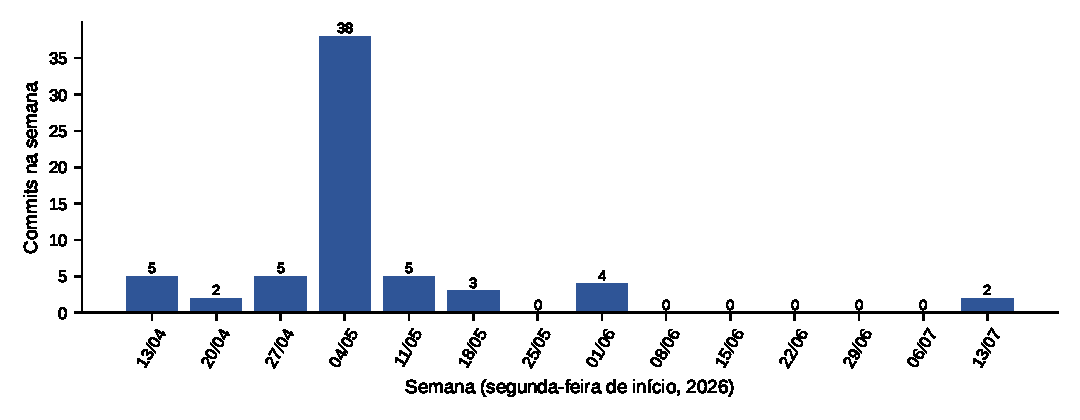
\includegraphics[width=0.9\textwidth]{figuras/commits_semana.pdf}
\fonte{Elaborado pela equipe (2026), a partir do histórico de \textit{commits}.}
\end{figure}

{\small
\begin{longtable}{|p{0.9cm}|p{2.1cm}|p{6.6cm}|p{2.6cm}|p{1.6cm}|}
\caption{Incrementos de desenvolvimento}\label{tab:incrementos}\\
\hline
\textbf{Inc.} & \textbf{Período} & \textbf{Objetivo e entregas} & \textbf{Evidência (\textit{commits})} & \textbf{Requisitos} \\ \hline
\endfirsthead
\hline
\textbf{Inc.} & \textbf{Período} & \textbf{Objetivo e entregas} & \textbf{Evidência (\textit{commits})} & \textbf{Requisitos} \\ \hline
\endhead
I0 & 16--21/04 (7 \textit{commits}) & \textbf{Exploração.} Protótipo de monitoramento TCP/HTTP, captura de tráfego em arquivo de pacotes com relatório em \textit{script} Python e tentativa de configuração por regras de \textit{firewall}. Primeira versão do analisador. & 743885b, d47a2d8, 1236bda, 6cebe4b, 2d8a085, 4de235e & --- \\ \hline
I1 & 29--30/04 (3) & \textbf{Primeira versão funcional.} Analisador por expressões regulares, registro de auditoria em arquivo, métricas e primeira documentação. Remoção do protótipo de captura de pacotes. & 8523640, 913d304, 7a7a1f1 & RF10, RF13, RF15 \\ \hline
I2 & 01--03/05 (2) & \textbf{CA local e configuração.} Geração da CA e instalação no macOS; leitura de configuração YAML com padrões personalizados e primeiro filtro de requisições. & 3683963, bdb96f0 & RF02, RF03, RF12, RF17 \\ \hline
I3 & 04/05 (9) & \textbf{Unificação e infraestrutura.} Consolidação do repositório; \textit{Makefile}; instaladores de CA para Linux e Windows; licença; \textit{workflow} de publicação; especificação do certificado. & 3fc3d71, 9317162, 93ab52a, c23afe3, 3964fb7 & RF03, RF24 \\ \hline
I4 & 05/05 (6) & \textbf{Testes de desempenho e de padrões.} \textit{Benchmark}, testes de latência e de vazão, testes de padrões personalizados e ajustes do exemplo de configuração. & ef79c09, 5bd4a00, 2d9942e, 18832a7, 7b154ff & RNF01, RNF03 \\ \hline
I5 & 06--08/05 (23) & \textbf{Integração, endurecimento e documentação.} Integração com uma segunda ferramenta de linha de comando; política de segurança e guia de contribuição; arquivo de proxy personalizado; instalação automática da CA no Linux; diagnóstico; comandos \textit{make}; desinstalação da CA; modo \textit{dry-run}; seção de riscos de segurança. & f629dd8, cd10441, 6f77577, d2c13a7, ea07ba6, 2be8767, 81de42e, aee374a, f3b3051 & RF03, RF14, RF21, RF22 \\ \hline
I6 & 12--18/05 (8) & \textbf{Refatoração do proxy.} Identificação de requisições de IA pelo corpo, inferência de provedor, modos \textit{whitelist} e \textit{passive}, limite de corpo e 370 linhas de testes de filtro; correções de CI; ajustes de documentação e demonstração. & 6a234ce, bb9872f, 8ad5a6e, 98dfe25 & RF05--RF09 \\ \hline
I7 & 02--03/06 (4) & \textbf{Interface de linha de comando e TUI.} Subcomandos e \textit{flags}; painel em tempo real; edição de padrões e do proxy com persistência no YAML; \textit{script} de instalação para Windows; pré-lançamento. & 0982721, 72e0282, 925bbc4, 0a1158e & RF18--RF20, RF24 \\ \hline
I8 & 17/07 (2) & \textbf{Distribuição e limpeza.} Documentação da instalação por Homebrew e remoção de arquivos sem uso. & 137478e, faebae9 & RF24 \\ \hline
\end{longtable}
}
\noindent\fonte{Elaborado pela equipe (2026), a partir do histórico de versionamento.}

Três observações caracterizam o processo. Primeiro, o incremento I0 foi um \textit{spike} exploratório cuja principal contribuição foi negativa: a captura passiva de pacotes não permite inspecionar o conteúdo de tráfego TLS, o que motivou a adoção do proxy com terminação TLS (decisão D01, Seção~\ref{sec:dev_decisoes}). Segundo, houve uma concentração de esforço em 4--8 de maio (38 dos 64 \textit{commits}), com predominância de infraestrutura e documentação. Terceiro, os requisitos centrais (RF10 a RF13) foram entregues cedo (I1), e os incrementos seguintes ampliaram a abrangência (I6), a operacionalidade (I3, I5) e a usabilidade (I7), o que é coerente com a priorização MoSCoW do Capítulo~\ref{chp:req}.

\section{Reuniões de Acompanhamento}
\label{sec:dev_reunioes}

O acompanhamento com a orientação é registrado em formato de ata resumida, com data, pauta, deliberações e encaminhamentos. A Tabela~\ref{tab:reunioes} reúne as orientações recebidas que já foram incorporadas ao trabalho e reserva linhas para as demais reuniões.

\begin{table}[htb]
\centering
\caption{Registro de reuniões de acompanhamento e orientações incorporadas}\label{tab:reunioes}
\small
\begin{tabular}{|p{1.8cm}|p{3.3cm}|p{5.2cm}|p{3.6cm}|}
\hline
\textbf{Data} & \textbf{Pauta} & \textbf{Deliberação / orientação} & \textbf{Encaminhamento} \\ \hline
\ 27/08/2026 & Critérios da revisão da literatura & Todas as referências devem possuir DOI ou ISSN; excluir TCCs e documentos sem revisão por pares. & Aplicado à seleção e ao arquivo de referências (Capítulo~\ref{chp:fund}). \\ \hline
\ 27/08/2026 & Justificativa do problema & Fundamentar o trabalho com casos reais de vazamento de dados. & Casos incluídos no Capítulo~\ref{chp:fund}; ampliar com fontes revisadas por pares. \\ \hline
\ 27/08/2026 & Apresentação da solução & Não nomear o produto antes do capítulo de resultados. & Texto dos Capítulos~\ref{chp:req} a~\ref{chp:test} usa descrição genérica. \\ \hline

\end{tabular}
\fonte{Elaborado pela equipe (2026).}
\end{table}


\section{Registro das Decisões}
\label{sec:dev_decisoes}

As decisões técnicas relevantes são registradas no formato de \textit{architecture decision records} simplificados: contexto e decisão, alternativas e justificativa, e consequências. Cada decisão aponta para o \textit{commit} em que se tornou observável no código. As justificativas foram reconstruídas a partir do código, do histórico e da documentação do projeto.



{\small
\begin{longtable}{|p{1.0cm}|p{4.2cm}|p{5.4cm}|p{3.3cm}|}
\caption{Registro de decisões técnicas}\label{tab:adr}\\
\hline
\textbf{ID} & \textbf{Decisão} & \textbf{Alternativas e justificativa} & \textbf{Consequências} \\ \hline
\endfirsthead
\hline
\textbf{ID} & \textbf{Decisão} & \textbf{Alternativas e justificativa} & \textbf{Consequências} \\ \hline
\endhead
D01  & Interceptar o tráfego por proxy com terminação TLS, em vez de captura passiva de pacotes ou regras de \textit{firewall}. & A captura passiva (testada em I0) observa apenas tráfego cifrado e não permite ler nem alterar o corpo; regras de \textit{firewall} só permitem bloquear. O proxy com terminação TLS é a única das alternativas que permite detectar e redigir o conteúdo. & Exige instalar e confiar numa CA local (D04) e não funciona com clientes que fixam certificados. \\ \hline
D02  & Implementar em Go. & Alternativas: linguagens com máquina virtual ou interpretadas. Go entrega binário estático multiplataforma, com biblioteca padrão para HTTP, TLS e X.509. & Distribuição simples (RNF07); dependência de biblioteca de proxy de terceiros. \\ \hline
D03  & Detectar dados sensíveis por expressões regulares e valores literais, sem classificadores de aprendizado de máquina. & Os trabalhos revisados usam modelos para reduzir falsos positivos em artefatos estáticos \cite{rahman2025secret,tsebak2025enhancing}; no caminho crítico de cada requisição, a abordagem determinística tem custo previsível, sem dependências nem inferência, e é auditável. & Cobertura limitada aos formatos conhecidos ou configurados; a evolução natural é um estágio híbrido, como o proposto nesses trabalhos. \\ \hline
D04  & Gerar uma CA exclusiva na máquina do usuário (RSA 4096, 10 anos), instalá-la no repositório do sistema e nunca versioná-la. & Alternativas: CA compartilhada distribuída com o produto (rejeitada: a chave comprometida afetaria todos os usuários) ou desativar a verificação de certificados nos clientes (rejeitada: reduz a segurança). & O usuário concede confiança à CA; a chave local torna-se ativo crítico (RNF04). \\ \hline
D05  & Configuração por arquivo YAML opcional, com padrões embutidos ativos por omissão. & Alternativas: \textit{flags} apenas ou banco de dados. O YAML é legível, versionável e editável por humanos; o funcionamento sem arquivo reduz a barreira de adoção. & Sem recarga a quente: mudanças valem na próxima inicialização. \\ \hline
D06  & Persistir a auditoria em arquivo JSON Lines, sem SGBD. & Alternativas: banco embarcado ou servidor. O arquivo de inclusão atende ao requisito de binário único e é consumível por ferramentas externas (Seção~\ref{sec:proj_dados}). & Consultas analíticas exigem ferramentas externas; proposta relacional na Seção~\ref{sec:proj_relacional}. \\ \hline
D07  & Identificar requisições de IA pelo conteúdo do corpo, e oferecer os modos \textit{whitelist} e \textit{passive}. & Alternativa: lista fixa de \textit{hosts} dos provedores (rejeitada: não cobre novas ferramentas e provedores). A identificação por corpo sustenta o agnosticismo (RNF11); o modo \textit{whitelist} reduz o escopo quando se conhecem os destinos. & Possibilidade de falsos positivos de classificação em corpos JSON com campos homônimos. \\ \hline
D08 & Oferecer modo \textit{dry-run}. & Permite validar padrões e calibrar a seletividade sem arriscar a integridade das requisições, mitigando o custo de adoção. & Requer comparar registros com e sem alteração. \\ \hline
D09  & Registrar auditoria e eventos de interface de forma assíncrona e não bloqueante, descartando eventos quando a fila está cheia. & Alternativa: gravação síncrona (rejeitada: acoplaria a latência da requisição ao disco). A prioridade é não degradar a experiência do desenvolvedor (RNF09). & Possível perda de registros sob sobrecarga; condição de corrida identificada no registrador (Seção~\ref{sec:test_problemas}). \\ \hline
D10  & Restringir a negociação TLS interceptada ao HTTP/1.1. & Evita o tratamento de HTTP/2 no \textit{pipeline}, mantendo o processamento restrito ao protocolo suportado pelo proxy. & Clientes que exijam HTTP/2 serão rebaixados ao negociar. \\ \hline
D11  & Prover TUI com a biblioteca Bubble Tea. & Alternativas: interface web local ou apenas linha de comando. A TUI mantém o produto em um único binário e no terminal em que a ferramenta já é usada. & Requer terminal com largura mínima de 80 colunas (RNF08). \\ \hline
D12  & Distribuir binários por \textit{workflow} de CI, com \textit{checksums}, e por Homebrew e \textit{script} PowerShell. & Mitiga o risco de comprometimento do binário (Seção~\ref{sec:proj_arq}) e simplifica a instalação por plataforma. & Manutenção de múltiplos canais de distribuição. \\ \hline
\end{longtable}
}
\noindent\fonte{Elaborado pela equipe (2026).}

\section{Atualizações da Documentação}
\label{sec:dev_doc}

A documentação evoluiu junto com o código: 36 dos 64 \textit{commits} alteraram o arquivo principal de documentação, e 23 mensagens de \textit{commit} referem-se explicitamente a documentação. Em duas ocasiões (\textit{commits} f2097ea e faebae9) foram removidos documentos temporários e desatualizados, o que reduziu a ambiguidade. A Tabela~\ref{tab:docs} lista os documentos mantidos e sua função.

\begin{table}[htb]
\centering
\caption{Documentação mantida no repositório}\label{tab:docs}
\small
\begin{tabular}{|p{4.4cm}|p{9.5cm}|}
\hline
\textbf{Documento} & \textbf{Conteúdo} \\ \hline
Documento principal & Instalação (Homebrew e binários), compilação, configuração da CA, comandos, modos do proxy, padrões, desempenho, auditoria, testes e \textit{roadmap}. \\ \hline
Política de segurança & Procedimento de relato de vulnerabilidades. \\ \hline
Guia de contribuição & Pré-requisitos, estratégia de ramos, diretrizes de código, testes e processo de \textit{pull request}. \\ \hline
Exemplo de configuração & Arquivo YAML comentado com todos os campos. \\ \hline
Esquema de auditoria & Descrição campo a campo do registro de auditoria. \\ \hline
Guia de execução de testes & Comandos para cada teste automatizado. \\ \hline
Roteiro de testes manuais & Cenários de validação ponta a ponta com ferramenta de IA. \\ \hline
\end{tabular}
\fonte{Elaborado pela equipe (2026).}
\end{table}

A revisão realizada para esta entrega identificou divergências entre a documentação e o código, descritas na Seção~\ref{sec:test_problemas} (itens P10 a P14). Elas constituem a lista de atualizações pendentes da documentação: corrigir o esquema de auditoria, harmonizar a versão da linguagem, atualizar o roteiro de testes manuais (que cita caminho de máquina específico e comportamento de \textit{streaming} não implementado), revisar a tabela de padrões suportados e a descrição do provedor inferido, e alinhar o guia de contribuição aos ramos existentes.
 % Desenvolvimento da solução
\chapter{Testes e Validação}\label{chp:test}

Este capítulo apresenta o planejamento dos testes, os casos de teste, a execução com o registro das evidências, os problemas encontrados e o plano de validação com usuários. A verificação confronta o comportamento observado do mecanismo com os requisitos do Capítulo~\ref{chp:req}; a validação, que avalia se o mecanismo é útil e aceitável para quem o usa, é planejada na Seção~\ref{sec:test_usuarios}.

\section{Planejamento dos Testes}
\label{sec:test_plano}

\subsection{Objetivos e níveis}

Os testes têm três objetivos: (i) verificar os requisitos funcionais críticos (RF01 a RF17) e os requisitos não funcionais mensuráveis (RNF01 a RNF03, RNF09); (ii) obter evidências de desempenho que sustentem a avaliação de impacto operacional, que é uma das contribuições da pesquisa; e (iii) identificar defeitos antes da etapa de experimentação. Foram definidos quatro níveis:

\begin{description}
    \item[N1 -- Unitário automatizado.] Testes com o pacote de testes da linguagem sobre o analisador, o filtro, a inferência de provedor, a configuração e a interface de terminal.
    \item[N2 -- Desempenho.] Medições de latência e de vazão do analisador, com cargas de tamanhos variados.
    \item[N3 -- Integração e sistema.] Execução do proxy completo, com cliente e destino reais ou simulados, exercitando o \textit{pipeline} de ponta a ponta e a trilha de auditoria.
\end{description}

\subsection{Ambiente, dados e critérios}

\textbf{Ambiente de verificação.} A execução registrada neste capítulo foi realizada em 14 de outubro de 2026, sobre a versão do código correspondente ao \textit{commit} faebae9, em ambiente Linux (Ubuntu 24.04, amd64), compilador Go 1.24.13 e processador Intel Xeon de 2,1~GHz. Como o módulo declara a versão 1.25 da linguagem, a verificação foi feita em uma cópia descartável com a diretiva ajustada para 1.24, e as dependências foram resolvidas a partir das versões fixadas no módulo; o código-fonte do repositório não foi modificado. A interface de terminal (N1) não pôde ser executada por exigir bibliotecas que não foram resolvidas nesse ambiente.


\textbf{Dados de teste.} Todos os segredos usados são fictícios, com o formato dos \textit{tokens} reais e sem validade. Nenhum teste utiliza credenciais ou código de terceiros.

\textbf{Critérios de aceitação.} (i) todos os testes automatizados aprovados; (ii) nenhum falso positivo nos casos benignos (RNF03); (iii) latência média do analisador inferior a 3~ms para corpos de até 1~MiB (RNF01); (iv) requisição redigida mantida íntegra (JSON válido e tamanho declarado coerente); (v) nenhum defeito de severidade alta em aberto ao final da etapa.

\textbf{Riscos do plano.} A cobertura de testes automatizados do pacote central é parcial (Seção~\ref{sec:test_exec}); o comportamento com ferramentas de IA reais e com HTTPS depende de testes manuais por plataforma; e o desempenho medido em um equipamento não se generaliza para outros.

\section{Casos de Teste}
\label{sec:test_casos}

\subsection{Testes automatizados existentes}

A Tabela~\ref{tab:suites} agrupa os testes automatizados do repositório, associando-os aos requisitos que verificam. A coluna \textit{Testes} indica a quantidade de funções de teste de primeiro nível; os testes parametrizados executam subtestes adicionais.

\begin{table}[htb]
\centering
\caption{Suítes de teste automatizadas}\label{tab:suites}
\small
\begin{tabular}{|p{1.3cm}|p{5.9cm}|p{1.6cm}|p{2.2cm}|p{2.4cm}|}
\hline
\textbf{ID} & \textbf{O que verifica} & \textbf{Testes} & \textbf{Requisitos} & \textbf{Nível} \\ \hline
CT-A01 & Detecção correta de cada formato de credencial embutido (16 casos). & 1 & RF10 & N1 \\ \hline
CT-A02 & Ausência de falsos positivos em 32 dados benignos (identificadores, \textit{hashes}, Base64, URLs, nomes de métodos, \textit{tokens} de outros serviços). & 1 & RNF03 & N1 \\ \hline
CT-A03 & Padrões personalizados por expressão regular (senha de banco, \textit{string} de conexão, JWT, chave privada). & 1 & RF12 & N1 \\ \hline
CT-A04 & Padrões personalizados literais (tabelas internas, nomes de projetos). & 1 & RF12 & N1 \\ \hline
CT-A05 & Ausência de falsos positivos em 10 entradas benignas para padrões personalizados. & 1 & RF12, RNF03 & N1 \\ \hline
CT-A06 & Latência do analisador (7 cargas $\times$ 1000 iterações), falhando se a média ultrapassar 3~ms. & 1 & RNF01 & N2 \\ \hline
CT-A07 & Vazão do analisador. & 1 & RNF01 & N2 \\ \hline
CT-A08 & Leitura, escrita e \textit{round-trip} da configuração YAML; padrões, porta por omissão e erro para YAML inválido ou caminho sem permissão. & 7 & RF11, RF12, RF17 & N1 \\ \hline
CT-A09 & Casamento de curingas de \textit{host}, tipo de conteúdo e função de classificação de provedores. & 6 & RF06, RF07 & N1 \\ \hline
CT-A10 & Reconhecimento de requisições de IA por formato de provedor, vazias ou inválidas (9 testes) e decisão de processamento por método, tipo, \textit{host} e modo (8 testes). & 17 & RF05--RF08 & N1 \\ \hline
CT-A11 & Inferência de provedor e modelo a partir do corpo. & 7 & RF09 & N1 \\ \hline
CT-A12 & Contadores, anel de eventos, telas e navegação da TUI. & 21 & RF18--RF20 & N1 \\ \hline
\end{tabular}
\fonte{Elaborado pela equipe (2026).}
\end{table}

\subsection{Casos de teste de integração e de sistema}

Os casos da Tabela~\ref{tab:integracao} exercitam o proxy completo. Foram elaborados a partir do roteiro de testes manuais do repositório e automatizados em um teste de integração que inicia o proxy, um destino HTTP simulado que devolve o corpo recebido e um cliente configurado para usar o proxy. Os casos CT-M01 a CT-M07, que dependem de plataforma, de ferramenta real ou de interação humana, permanecem como testes manuais.

\begin{table}[htb]
\centering
\caption{Casos de teste de integração e de sistema}\label{tab:integracao}
\small
\begin{tabular}{|p{1.35cm}|p{4.4cm}|p{5.6cm}|p{2.3cm}|}
\hline
\textbf{ID} & \textbf{Cenário} & \textbf{Resultado esperado} & \textbf{Requisitos} \\ \hline
CT-I01 & Requisição de IA com chave de projeto e chave de acesso AWS fictícias no \textit{prompt}. & Destino recebe as chaves substituídas pelo rótulo; JSON válido; tamanho declarado coerente. & RF01, RF08, RF10, RF13 \\ \hline
CT-I02 & Requisição de IA sem dado sensível. & Corpo entregue idêntico ao enviado. & RF13, RNF03 \\ \hline
CT-I03 & JSON sem campos de requisição de IA contendo chave fictícia. & Requisição ignorada e entregue sem alteração (comportamento por projeto). & RF08 \\ \hline
CT-I04 & Requisição \texttt{POST} com tipo de conteúdo texto simples. & Requisição ignorada e entregue sem alteração. & RF05 \\ \hline
CT-I05 & Modo \textit{dry-run} com chave fictícia. & Corpo idêntico ao original; evento registrado como detecção. & RF14 \\ \hline
CT-I06 & \textit{Host} presente na lista de ignorados. & Corpo idêntico ao original. & RF07 \\ \hline
CT-I07 & Modo \textit{whitelist} com \textit{host} fora da lista de permitidos. & Corpo idêntico ao original. & RF06 \\ \hline
CT-I08 & Destino inalcançável. & Erro explícito devolvido ao cliente, sem travamento do proxy. & RF16, RNF09 \\ \hline
CT-I09 & Corpo de 6~MiB (acima do limite de análise). & Requisição encaminhada íntegra ou rejeitada de forma explícita. & RF05, RNF02 \\ \hline
CT-I10 & 100 requisições concorrentes com chave fictícia. & Todas atendidas e uma entrada de auditoria por requisição; trilha sem segredos. & RNF09, RNF10, RF15 \\ \hline
CT-M01 & Instalação da CA em macOS, Linux e Windows. & CA confiável pelo sistema; diagnóstico indica ``instalado''. & RF02, RF03 \\ \hline
CT-M02 & Ferramenta de IA real configurada para o proxy, com HTTPS. & Funcionamento normal da ferramenta e redação observada na auditoria. & RF04, RNF11 \\ \hline
CT-M03 & Uso da TUI: painel, criação e exclusão de padrão, edição do proxy. & Telas navegáveis; alterações gravadas no arquivo. & RF18--RF20 \\ \hline
CT-M04 & Execução de \texttt{doctor}, \texttt{version} e \texttt{help}. & Saídas conforme o esperado. & RF21, RF22 \\ \hline
CT-M05 & Encerramento por sinal durante tráfego. & Registro de auditoria persistido sem corrupção. & RF23 \\ \hline
CT-M06 & Conexão mantida aberta além do limite de tempo. & Conexão encerrada de forma controlada. & RNF09 \\ \hline
CT-M07 & Instalação por Homebrew e por binário, com verificação de \textit{checksum}. & Binário executável; \textit{checksum} confere. & RF24, RNF07 \\ \hline
\end{tabular}
\fonte{Elaborado pela equipe (2026), a partir do roteiro de testes do repositório.}
\end{table}

\section{Execução e Registro de Evidências}
\label{sec:test_exec}

\subsection{Procedimento}

Os comandos executados são apresentados no Listagem~\ref{lst:cmds}. A opção de detecção de corridas de dados foi incluída por ser adequada a um sistema com várias \textit{goroutines} (servidor, \textit{workers} de auditoria e interface).

\begin{lstlisting}[basicstyle=\ttfamily\scriptsize, frame=single, caption={Comandos de execução dos testes}, label={lst:cmds}, captionpos=t, breaklines=true]
go test -v -count=1 ./...                         # suites automatizadas
go test -count=1 -cover ./internal/guardian/      # cobertura do pacote central
go test -race -count=1 ./...                      # deteccao de corridas de dados
go test -run xxx -bench . -benchmem ./internal/guardian/   # benchmarks
\end{lstlisting}

\subsection{Resultados dos testes automatizados}

O pacote central (analisador, filtro, provedor, configuração e auditoria) executou 44 testes de primeiro nível e 52 subtestes, todos aprovados, com cobertura de 31,8\% das instruções; o detector de corridas, aplicado à suíte existente, não reportou ocorrências. A análise estática do pacote (\texttt{go vet}) não emitiu avisos. Os casos CT-A02 e CT-A05 resultaram em 0 falso positivo em 32 e em 10 entradas, respectivamente. A baixa cobertura decorre de o manipulador de requisições do proxy, a auditoria e os pacotes de CA e de diagnóstico não possuírem testes automatizados; esse é o principal vazio do plano (Tabela~\ref{tab:rastreio}).

\subsection{Resultados dos testes de integração}

A Tabela~\ref{tab:res_int} apresenta os resultados dos casos CT-I01 a CT-I10, obtidos com o proxy completo e um destino simulado.

\begin{table}[htb]
\centering
\caption{Resultados dos casos de integração (14/10/2026)}\label{tab:res_int}
\small
\begin{tabular}{|p{1.35cm}|p{9.6cm}|p{2.5cm}|}
\hline
\textbf{ID} & \textbf{Observação} & \textbf{Resultado} \\ \hline
CT-I01 & Ambas as chaves foram substituídas pelo rótulo; o JSON permaneceu válido e o tamanho declarado coincidiu com o corpo entregue. & Aprovado \\ \hline
CT-I02 & Corpo entregue idêntico. & Aprovado \\ \hline
CT-I03 & Corpo entregue sem alteração; a chave fictícia \textbf{não} foi redigida por o JSON não conter campos de IA. & Conforme o projeto; limitação \\ \hline
CT-I04 & Corpo entregue sem alteração. & Aprovado \\ \hline
CT-I05 & Corpo idêntico ao original; evento registrado com as detecções. & Aprovado \\ \hline
CT-I06 & Corpo idêntico. & Aprovado \\ \hline
CT-I07 & Corpo idêntico. & Aprovado \\ \hline
CT-I08 & O cliente recebeu resposta de erro (status 500), e o proxy continuou operante. & Aprovado, com ressalva \\ \hline
CT-I09 & Foram enviados 6.291.516 bytes e o destino recebeu 5.242.880 (exatamente 5~MiB), com JSON inválido: a requisição é truncada (P02). & \textbf{Reprovado} \\ \hline
CT-I10 & 99 das 100 requisições concorrentes foram atendidas; a trilha registrou 108 das 109 entradas esperadas no cenário completo; nenhuma entrada contém segredo. A causa da falha isolada não foi investigada. Com o detector de corridas, o teste de integração acusou corridas de dados. & \textbf{Reprovado} \\ \hline
\end{tabular}
\fonte{Elaborado pela equipe (2026).}
\end{table}

\subsection{Resultados de desempenho}

O teste de latência do repositório, executado no ambiente de verificação, resultou em média de 0,95~\textmu s, P95 de 1,92~\textmu s e P99 de 5,06~\textmu s, valores da mesma ordem dos registrados na documentação do projeto (média de 1,07~\textmu s), obtidos em outro equipamento. No entanto, esse teste usa sete cargas de menos de cem bytes, muito menores que as requisições reais de assistentes de código, que carregam contexto de arquivos. Por isso foram realizadas medições complementares com corpos de 1~KB a 5~MiB, contendo código-fonte comum e os nove padrões embutidos ativos (Tabela~\ref{tab:desempenho}). Cada valor é a mediana de três execuções de \textit{benchmark}.

\begin{table}[htb]
\centering
\caption{Latência do analisador por tamanho de corpo (ambiente de verificação)}\label{tab:desempenho}
\small
\begin{tabular}{|p{4.6cm}|p{2.9cm}|p{2.7cm}|p{2.7cm}|}
\hline
\textbf{Carga} & \textbf{Tempo por operação} & \textbf{Vazão} & \textbf{Memória por operação} \\ \hline
1~KB & 2,4~\textmu s & 472 MB/s & 1,1~KB \\ \hline
10~KB & 22,7~\textmu s & 451 MB/s & 10,6~KB \\ \hline
100~KB & 0,22~ms & 474 MB/s & 104~KB \\ \hline
1~MiB & 2,44~ms & 429 MB/s & 1,0~MiB \\ \hline
5~MiB (limite de análise) & 13,5~ms & 388 MB/s & 5,0~MiB \\ \hline
100~KB, com duas credenciais a redigir & 0,28~ms & 371 MB/s & 314~KB (19 alocações) \\ \hline
\end{tabular}
\fonte{Elaborado pela equipe (2026).}
\end{table}

A análise cresce de forma aproximadamente linear com o tamanho do corpo, a cerca de 2,4~ms por MiB. Para corpos de até 1~MiB, o critério de RNF01 (média inferior a 3~ms) é atendido; no limite de 5~MiB, a análise leva cerca de 13,5~ms, valor ainda pequeno diante do tempo de resposta de um LLM, que costuma ser de segundos, mas acima do limiar do teste automatizado. A vazão de aproximadamente 400 a 500~MB/s indica que o analisador não é o gargalo do \textit{pipeline}. Duas ressalvas metodológicas sobre as medições do repositório são tratadas como problema P09.

\subsection{Evidências adicionais documentadas no repositório}

O repositório documenta, com capturas de tela, resultados de execução em um equipamento com processador Intel Core i5-13400 (Linux): detecção de todos os formatos de credencial, ausência de falsos positivos nos casos benignos, e resultados dos padrões personalizados (cinco de cinco para senha de banco, \textit{string} de conexão e chave privada; um de um para JWT; cinco de cinco para os literais de tabelas e de projetos).


\subsection{Modelo de registro de evidências}

Para as execuções futuras, cada rodada é registrada com os campos da Tabela~\ref{tab:modelo_ev}. As execuções de 14/10/2026 correspondem à primeira linha.

\begin{table}[htb]
\centering
\caption{Modelo de registro de execução de testes}\label{tab:modelo_ev}
\small
\begin{tabular}{|p{1.9cm}|p{2.1cm}|p{3.2cm}|p{2.6cm}|p{3.7cm}|}
\hline
\textbf{Data} & \textbf{Versão} & \textbf{Ambiente} & \textbf{Casos} & \textbf{Resultado e evidência} \\ \hline
14/10/2026 & faebae9 & Linux amd64, Go 1.24.13, Xeon 2,1 GHz & CT-A01 a A11; CT-I01 a I10; \textit{benchmarks} & 44 testes aprovados; 2 casos de integração reprovados; saída de teste arquivada \\ \hline
\end{tabular}
\fonte{Elaborado pelo autor (2026).}
\end{table}

\section{Problemas Identificados e Correções}
\label{sec:test_problemas}

A verificação e a revisão do código e da documentação identificaram os problemas da Tabela~\ref{tab:problemas}. A coluna \textit{Origem} distingue o que foi \textbf{confirmado por execução} do que foi identificado por \textbf{leitura do código}. A severidade é uma avaliação do autor, baseada no impacto sobre os requisitos. Todos permanecem em aberto na data desta entrega; as correções são o objeto do próximo incremento e cada uma deve gerar ao menos um caso de teste de regressão.

{\small
\begin{longtable}{|p{0.95cm}|p{5.0cm}|p{1.5cm}|p{1.7cm}|p{3.1cm}|p{1.2cm}|}
\caption{Problemas identificados}\label{tab:problemas}\\
\hline
\textbf{ID} & \textbf{Descrição} & \textbf{Origem} & \textbf{Severidade} & \textbf{Correção proposta} & \textbf{Req.} \\ \hline
\endfirsthead
\hline
\textbf{ID} & \textbf{Descrição} & \textbf{Origem} & \textbf{Severidade} & \textbf{Correção proposta} & \textbf{Req.} \\ \hline
\endhead
P01 & Condição de corrida no registrador de auditoria: cada gravação dispara outra \textit{goroutine} que lê e escreve a lista de entradas e o arquivo sem exclusão mútua, comprometendo a integridade da trilha. & Execução (detector de corridas) & Alta & Gravar sob a mesma exclusão mútua, ou usar escritor único com canal. Teste concorrente com \texttt{-race}. & RF15, RNF09 \\ \hline
P02 & Corpos acima de 5~MiB são lidos até o limite e a requisição é encaminhada truncada, produzindo requisição inválida. & Execução (CT-I09) & Alta & Encaminhar o corpo integral sem análise, ou rejeitar explicitamente. Teste de limite. & RF05, RNF02 \\ \hline
P03 & Durações são armazenadas em milissegundos inteiros; análises que levam microssegundos são registradas como zero, impedindo medir o custo a partir da trilha. & Execução (trilha) & Média & Registrar em microssegundos. & RNF01, RF15 \\ \hline
P07 & O diagnóstico considera uma variável de ambiente de porta que o proxy não utiliza (a porta vem do YAML), podendo reportar porta diferente da efetiva. & Leitura de código & Baixa & Unificar a fonte da porta. & RF21 \\ \hline
P08 & Edições feitas na TUI são gravadas no YAML, mas não são aplicadas ao proxy em execução. & Leitura de código & Baixa & Recarga da configuração ou aviso explícito de reinício. & RF19, RF20 \\ \hline
\end{longtable}
}
\noindent\fonte{Elaborado pela equipe (2026).}

\section{Rastreabilidade entre Requisitos e Testes}

A Tabela~\ref{tab:rastreio} relaciona cada requisito funcional aos casos que o verificam. Requisitos sem cobertura automatizada concentram-se nos componentes de CA, auditoria, diagnóstico, encerramento e distribuição, e serão tratados por novos casos no próximo incremento.

\begin{table}[htb]
\centering
\caption{Matriz de rastreabilidade requisitos--testes}\label{tab:rastreio}
\small
\begin{tabular}{|p{1.5cm}|p{4.7cm}|p{1.5cm}|p{4.7cm}|}
\hline
\textbf{Req.} & \textbf{Casos} & \textbf{Req.} & \textbf{Casos} \\ \hline
RF01 & CT-I01 a I10 & RF14 & CT-I05 \\ \hline
RF02, RF03 & CT-M01 (não executado) & RF15 & CT-I10 (inspeção da trilha) \\ \hline
RF04 & CT-M02 (não executado) & RF16 & CT-I08 \\ \hline
RF05 & CT-A10, CT-I04, CT-I09 & RF17 & CT-A08 \\ \hline
RF06 & CT-A10, CT-I07 & RF18--RF20 & CT-A12 (não executado), CT-M03 \\ \hline
RF07 & CT-A09, CT-A10, CT-I06 & RF21, RF22 & CT-M04 (não executado) \\ \hline
RF08 & CT-A10, CT-I03 & RF23 & CT-M05 (não executado) \\ \hline
RF09 & CT-A11 & RF24 & CT-M07 (não executado) \\ \hline
RF10 & CT-A01, CT-A02 & RF25 & --- \\ \hline
RF11, RF12 & CT-A03 a A05, CT-A08 & RNF01 & CT-A06, CT-A07, \textit{benchmarks} \\ \hline
RF13 & CT-I01, CT-I02 & RNF03 & CT-A02, CT-A05, CT-I02 \\ \hline
\end{tabular}
\fonte{Elaborado pela equipe (2026).}
\end{table}

\section{Síntese}

A verificação confirmou o funcionamento do núcleo de detecção e redação: os formatos de credencial suportados são detectados, não houve falsos positivos nos casos de teste, e a requisição redigida permanece válida. O custo de análise é baixo (da ordem de 2,4~ms por MiB) e não representa gargalo frente ao tempo de resposta de um LLM. Por outro lado, a execução revelou dois defeitos de severidade alta (P01 e P02) e limitações de medição (P03, P04 e P09) que afetam diretamente a avaliação de impacto operacional da pesquisa. Esses pontos definem o escopo do próximo incremento antes da etapa de experimentação.
 % Testes e validação
\chapter{Experimento e Coleta de Dados}\label{chp:exp}

Esta seção descreve o experimento e o processo de coleta de dados..... 

\section{Descrição do Experimento}

\section{Processo de coleta de dados}

\section{Resultados Obtidos}

\textbf{ATENÇÃO}
%
%SSDDSDFSFDF
%SFSDFDFFSF
%SFFFSDFF
%
%

\section{Survey}

Nesta etapa, foi aplicado um \textit{survey} que foi elaborado questões semi-estruturadas. Algumas destas questões, ficaram em aberto, de forma proposital para permitir que os entrevistados pudessem falar sobre o assunto da pesquisa, de uma forma mais livre, sem ficar limitados às alternativas das questões. 

O \textit{survey} seguiu as recomendações de análise de Kitchenham e Pfleeger~\cite{pfleeger2001principles}.

O objetivo de pesquisa do estudo foi:

\begin{enumerate}
    \item q1
    \item q2
\end{enumerate}


















...autor, ano de publicação, título do trabalho, objetivo, metodologia aplicada, principais resultados (Tabela 1).

\begin{table}[htbp] 
\centering
\caption{Caracterização das publicações selecionadas} \label{tabela-frameworks}
\begin{tabular}{|p{4cm}|p{4cm}|p{4cm}|p{4cm}|}
\hline
\textbf{TÍTULO DO TRABALHO AUTOR ANO DE PUBLICAÇÃO} & \textbf{OBJETIVO} & \textbf{METODOLOGIA} & \textbf{PRINCIPAIS RESULTADOS}\\ \hline 

Titulo
&
Objetivo
&
Estudo de campo.
&
Resultado.
\\ \hline	
Titulo

&
Objetivo

& 
Revisão de
literatura.

& 
Resultado.

\\ \hline
Titulo

& 
Objetivo

& 
Estudo de campo.
& 
Resultado.

\\ \hline
Titulo

& 
Objetivo

& 
Estudo de campo. 
& 
Resultado.

\\ \hline
Titulo
& 
Objetivo
& 
Estudo de campo. 
& 
Resultado.
\\ \hline
Titulo

& 
Objetivo
& 
Estudo de campo. 
& 
Resultado.
\\ \hline
\end{tabular}
\end{table}

Fonte:dados da pesquisa (2022).

 % Texto do cap4.tex
\chapter{Conclusões}\label{chp:conc}

\blindtext



\section{Trabalhos futuros}

\blindtext



 % Texto do cap5.tex



%%%%%%%%%%%%%%%%%%%%%%%%%%
%%Elementos Pós-Textuais%%
%%%%%%%%%%%%%%%%%%%%%%%%%%
%%--------Bibliografia--------
\Bibliografia{referenciasbibliograficas} % arquivo bibtex com as referências (referenciasbibliograficas.bib)

%%--------Apêndice--------
%% Descomente caso exista a necessidade da inclusão de apêndices
%\apendice % Comando que inclui os apêndices
%\include{7_Apendice/apendice_1}   % Arquivo apendice_1.tex
%\include{7_Apendice/apendice_2}   % Arquivo apendice_2.tex
%%---------------------------------------------------------------

%%--------Anexos-------------------------------------------------
%% Descomente caso exista a necessidade da inclusão de anexos
%\anexo % Comando que inclui os anexos (outros autores)
%\include{8_Anexos/anexo_1}  % Arquivo anexo_1.tex
%\include{8_Anexos/anexo_2}  % Arquivo anexo_2.tex
%%---------------------------------------------------------------
\appendix


\chapter{Apêndice}




\end{document}
